\documentclass[a4paper]{article}
\usepackage[a4paper, total={6in, 8in}]{geometry}
\usepackage[utf8]{inputenc}
\usepackage{courier}
\usepackage{minted}
\usepackage{pmboxdraw}
\usepackage{longtable}
\usepackage{array}
\usepackage{multirow}
\usepackage{graphicx}
\usepackage{wrapfig}
\usepackage{subcaption}
\usepackage{float}
\usepackage[bottom]{footmisc}
\usepackage{hyperref}

\graphicspath{ {./images/} }

\hypersetup{
    colorlinks=true,
    linkcolor=black,
    anchorcolor=black,
    citecolor=black,
    filecolor=black,
    menucolor=black,
    runcolor=black,
    urlcolor=blue,
}
\urlstyle{same}
\setminted{
fontsize=\footnotesize,
breaklines,
}

\renewcommand\arraystretch{1.3}
\setlength{\skip\footins}{5mm}

\renewcommand*\contentsname{Contenu}
\renewcommand{\refname}{Références}
\renewcommand{\listingscaption}{Extrait}


\begin{document}

\begin{titlepage}
   \begin{center}
        \vspace*{1cm}
        
        \Huge
        \textbf{Réalisation d'un jeu vidéo et de son serveur portable}
            
        \vspace{1.5cm}
        
        \LARGE
        Fabio Dubath \\
        Daniel Roulin
        \vspace{1.25cm}

\begin{figure}[h]
        \centering
        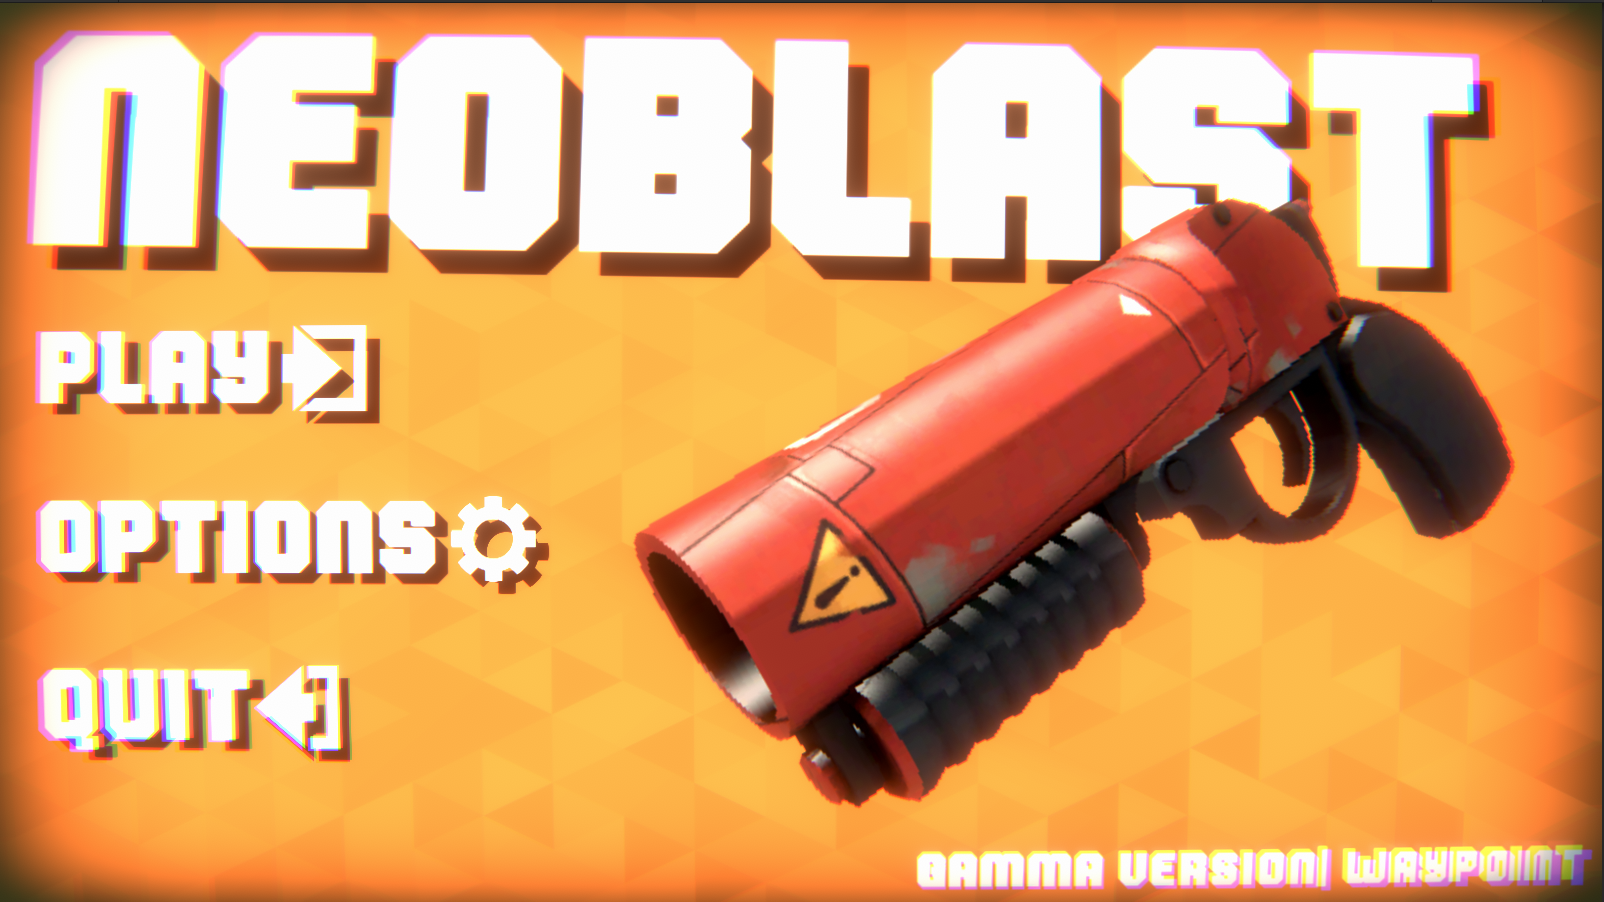
\includegraphics[width=0.9\textwidth]{images/game/start_menu.png}

\end{figure}

        \vfill
        
        \Large
        
        Supervisé par M. Daniel Kessler\\
        Collège André-Chavanne\\~\\
        2022
            
   \end{center}
\end{titlepage}

\newpage

\tableofcontents

\newpage

\section{Introduction}
Les jeux multijoueurs peuvent être classés en deux catégories: ceux qui se jouent sur le même appareil, sans connexion à internet, et ceux qui se jouent en ligne sur des appareils séparés. Cependant, il existe des situations où aucune de ces deux options ne sont viables. C'est pourquoi il nous est venu l'idée d'explorer une troisième configuration, celle de pouvoir jouer ensemble sur plusieurs appareils sans connexion à internet. Nous avons donc imaginé un boîtier, créant son propre réseau Wifi et permettant aux personnes environnantes de jouer simultanément, ainsi qu'un jeu adapté à cette nouvelle plateforme. Ce rapport documente la réalisation de ce projet.

\subsection{Les outils}
L’outil de base pour la création de notre jeu vidéo est le moteur de jeu Unity. Un moteur de jeu est une application contenant du code déjà en place qui enlève aux développeurs beaucoup de tâches fastidieuses comme le rendu des images sur l’écran ou encore l’exportation du jeu sur les différents systèmes d’exploitation. Unity a été publié en 2005 par Unity Technologies et permet de faire des jeux en 2D ou 3D, avec la possibilité d’exporter ces derniers sur une multitude de plateformes. Concernant le code, Unity utilise le langage C\#, qui est un langage de programmation orientée objet crée par Microsoft. Il est dérivé du C++ et est très proche du Java, dont il reprend la syntaxe générale ainsi que les concepts. Nous nous sommes aussi aidés de GitHub, qui est un service web d'hébergement et de gestion de développement de logiciels, utilisant le logiciel de gestion de versions Git \cite{git} ainsi que de l'outil d'organisation Trello \cite{trello} appartenant à Atlassian et basé sur le style Kanban.

\subsection{Le jeu}
Le concept du jeu est très simple. Les joueurs, dans une arène, ont accès à des armes et peuvent s’éliminer en se tirant dessus, ils réapparaissent une fois éliminés. Quand un joueur en élimine un autre, il gagne un point et celui qui a le plus de points à la fin du temps imparti a gagné. Le concept s'inspire du style   ``battle royale'', très populaire ces dernières années. \\
\\
Lorsque l'on démarre le jeu, on se retrouve sur le menu principal qui donne accès au menu de configuration, au bouton pour rejoindre le serveur et au bouton pour quitter le programme.

\begin{figure}[h]
    \begin{subfigure}{0.5\textwidth}
        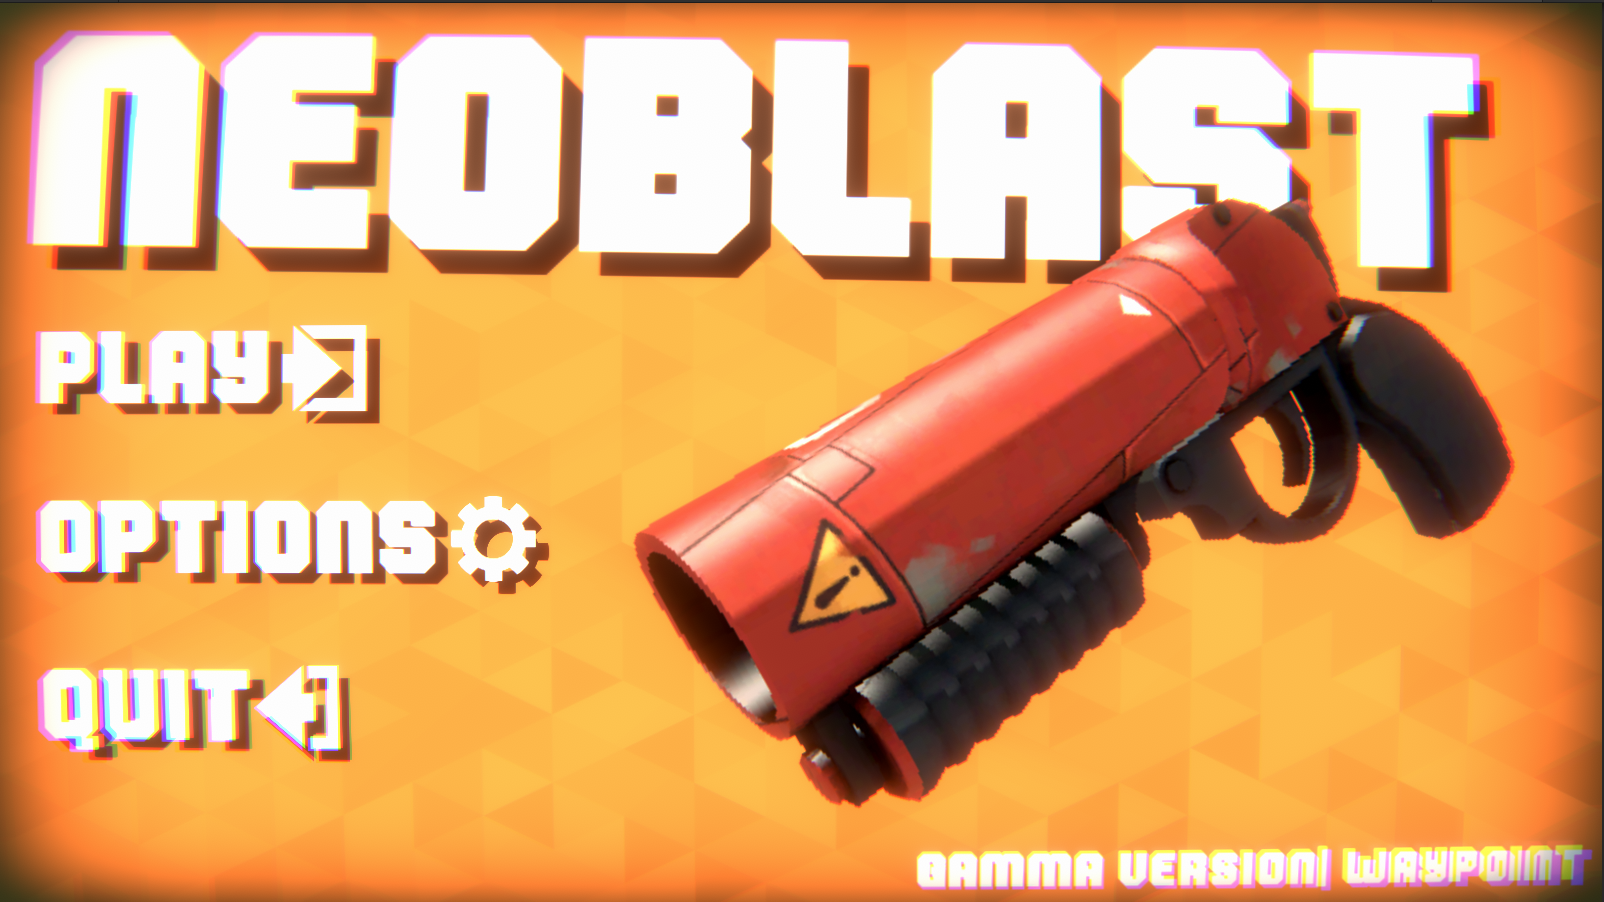
\includegraphics[width=0.9\textwidth]{images/game/start_menu.png}
        \caption{Menu de début de jeu}
        \label{fig:start_menu}
    \end{subfigure}
        \begin{subfigure}{0.5\textwidth}
        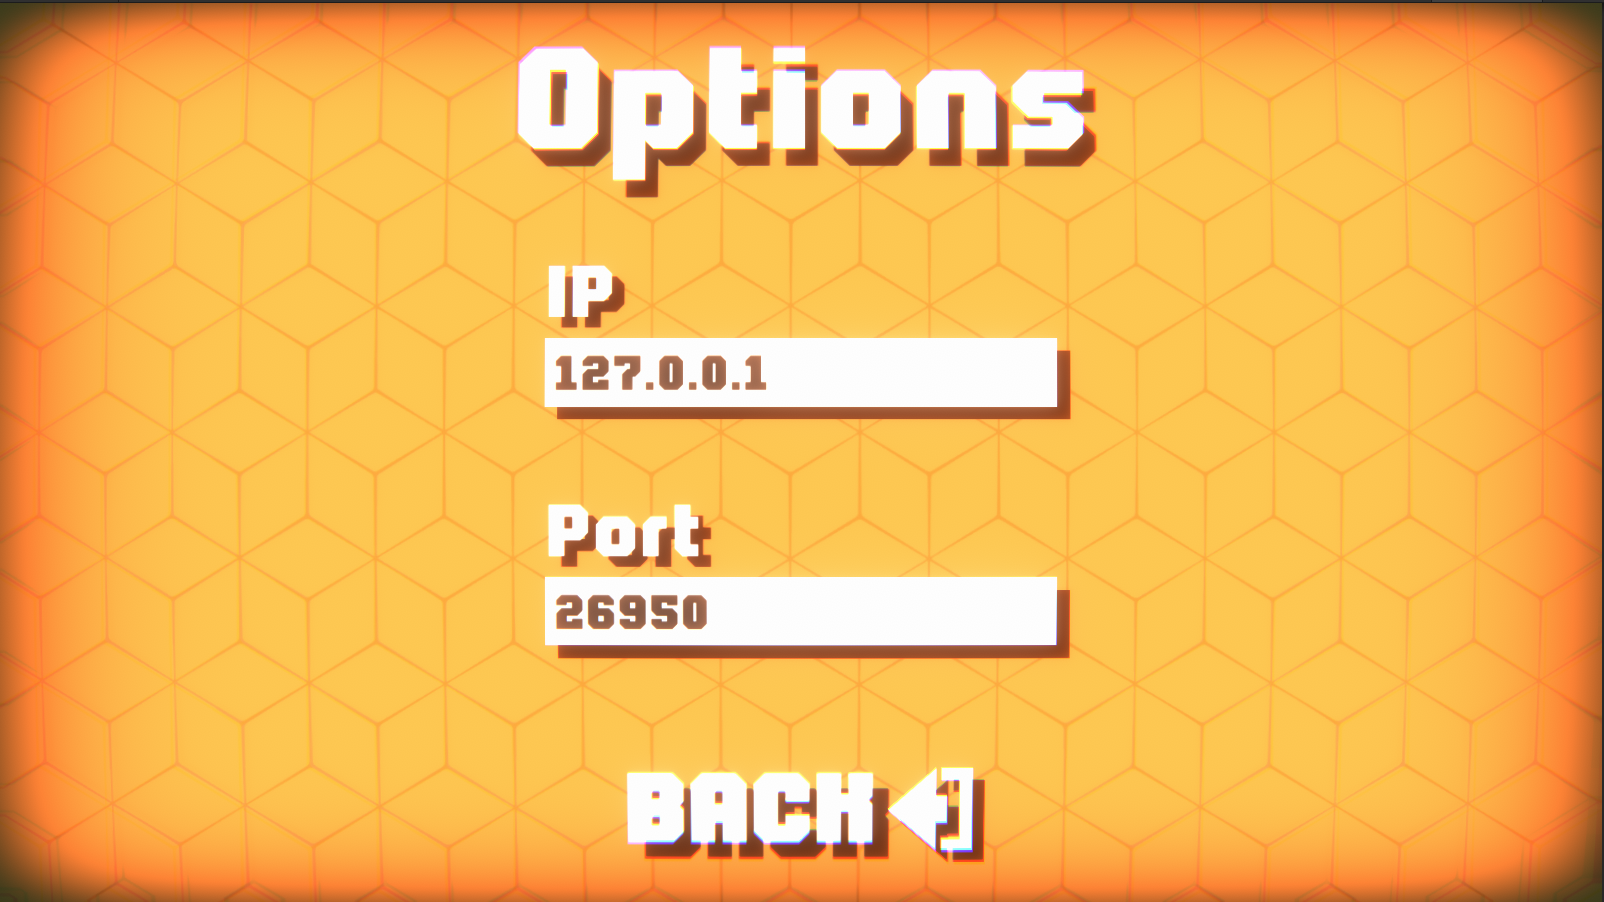
\includegraphics[width=0.9\textwidth]{images/game/option_menu.png}
        \caption{Menu de configuration}
        \label{fig:option_menu}
    \end{subfigure}
\end{figure}
\noindent Le menu de configuration permet à l'utilisateur de choisir l'adresse IP et le port du serveur sur lequel il veut se connecter, le programme indiquant si l'adresse insérée est valide.\\
\\
Une fois connecté, le joueur se retrouve dans la salle d'attente où il peut se déplacer et configurer son nom d'utilisateur le temps que tout le monde soit là. Quand les joueurs décident de démarrer la partie, ils se positionnent tous sur le carré "GO".

\begin{figure}[h]
    \begin{subfigure}{0.5\textwidth}
        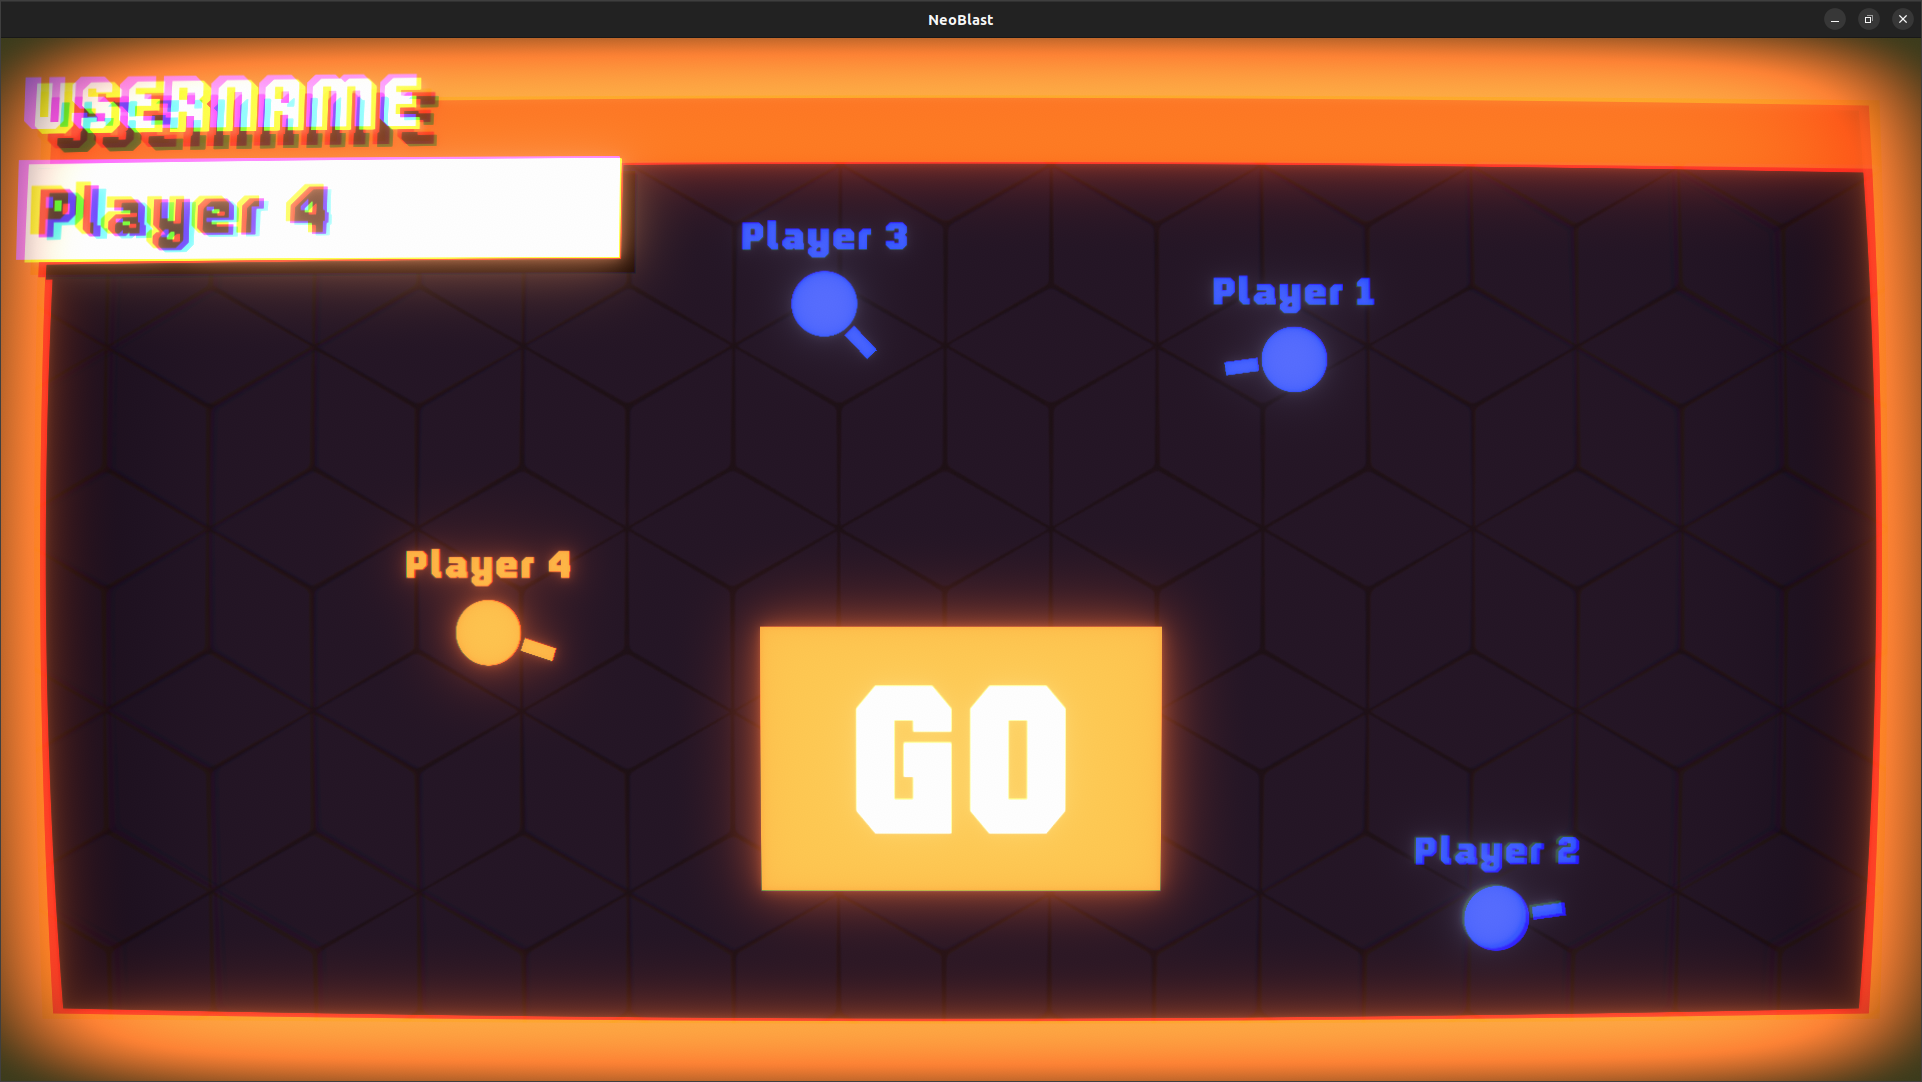
\includegraphics[width=0.9\textwidth, height = 4cm]{images/game/waiting_room.png}
        \caption{Salle d'attente}
        \label{fig:waiting_room}
    \end{subfigure}
        \begin{subfigure}{0.5\textwidth}
        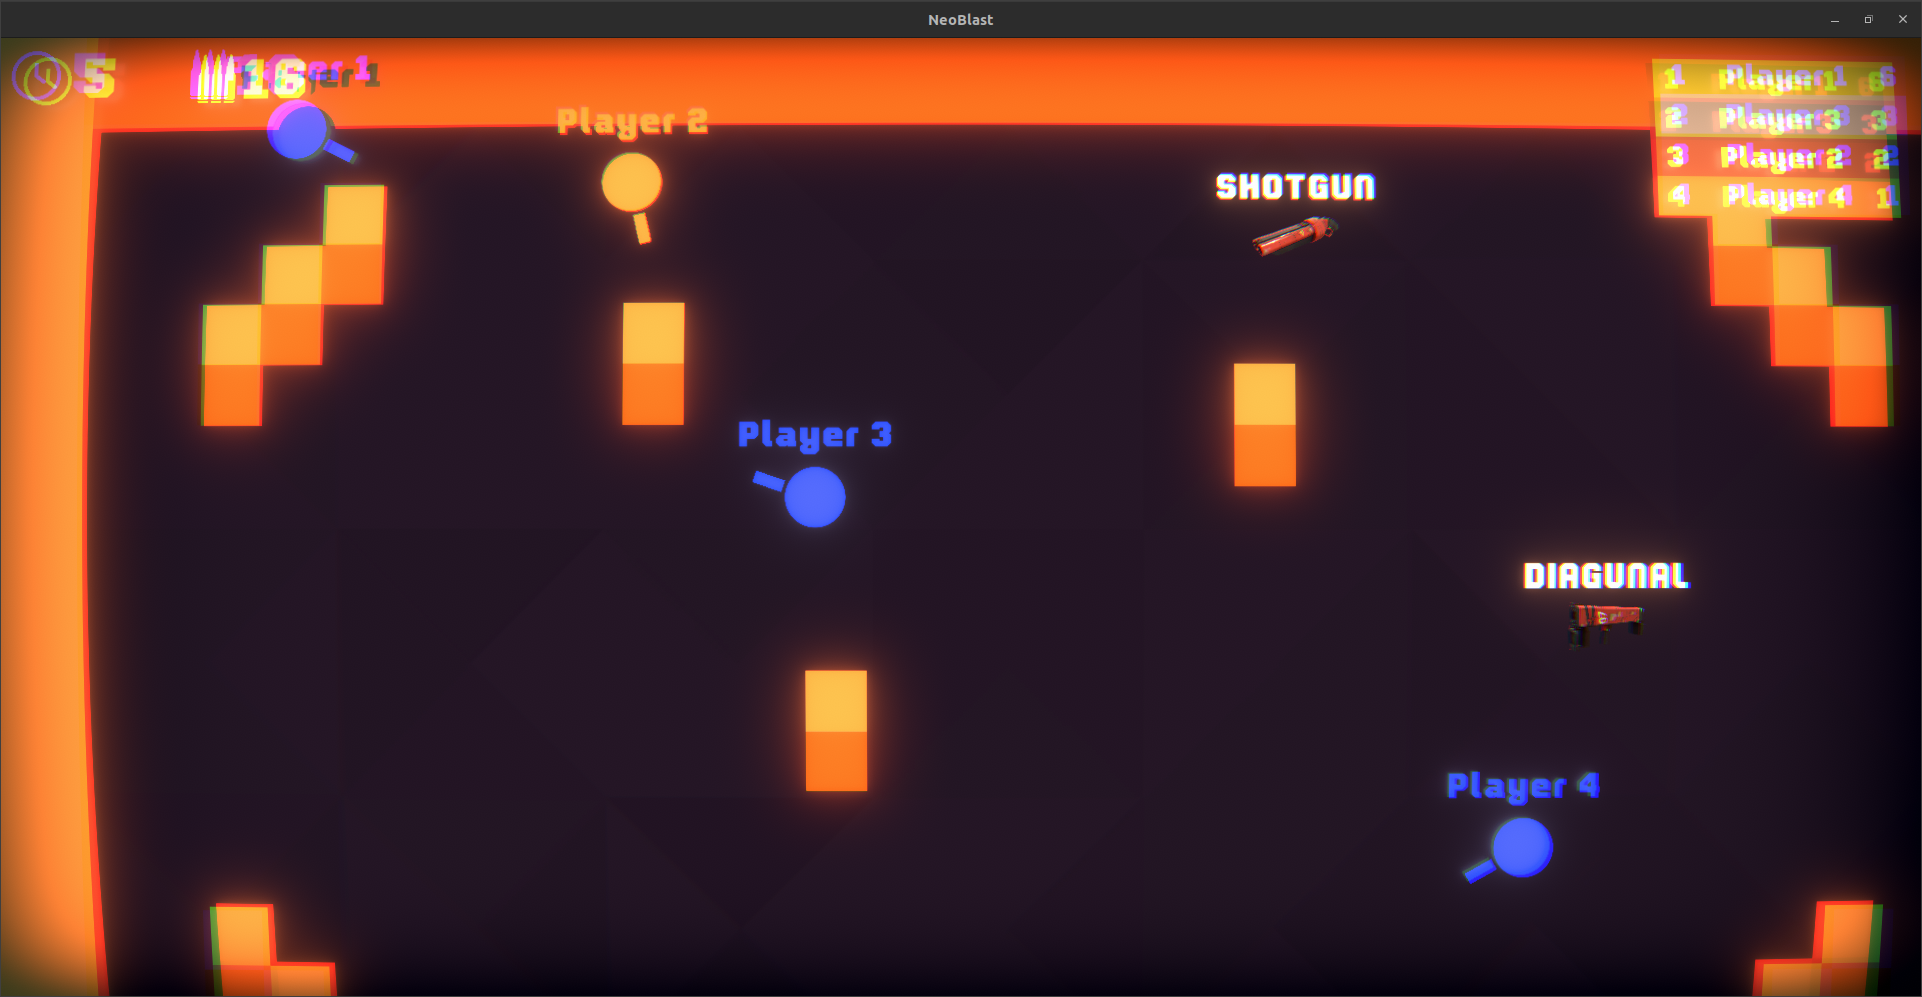
\includegraphics[width=0.9\textwidth, height = 4cm]{images/game/game.png}
        \caption{Jeu}
        \label{fig:jeu}
    \end{subfigure}
\end{figure}
\noindent Durant la partie, le joueur a accès au menu de pause qui lui permet de revenir au menu principal, mais qui ne met pas en pause la partie. Quand la partie est terminée, tous les joueurs sont emmenés au podium qui montre leur nombre d'éliminations. Puis, ils sont renvoyés vers la salle d'attente où une nouvelle partie peut être commencée.

\begin{figure}[h]
    \begin{subfigure}{0.5\textwidth}
        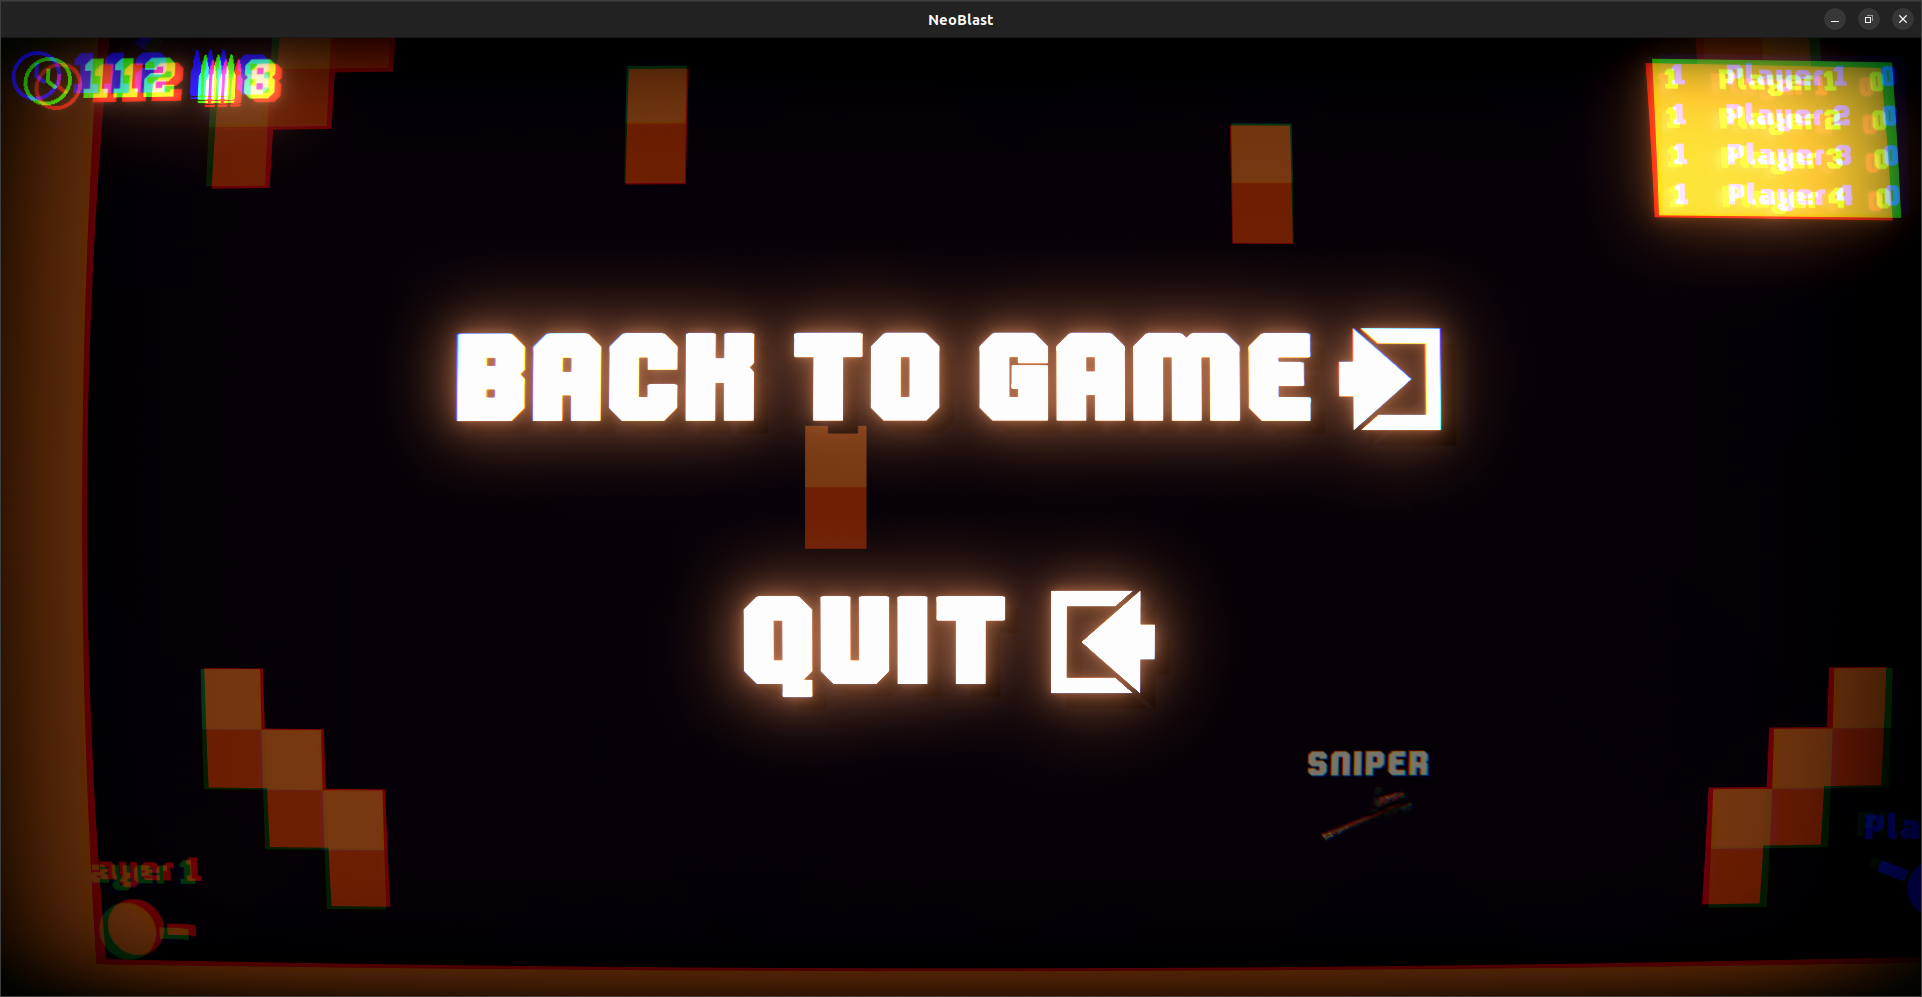
\includegraphics[width=0.9\textwidth, height = 4cm]{images/game/pause_menu.png}
        \caption{Menu de pause}
        \label{fig:pause_menu}
    \end{subfigure}
        \begin{subfigure}{0.5\textwidth}
        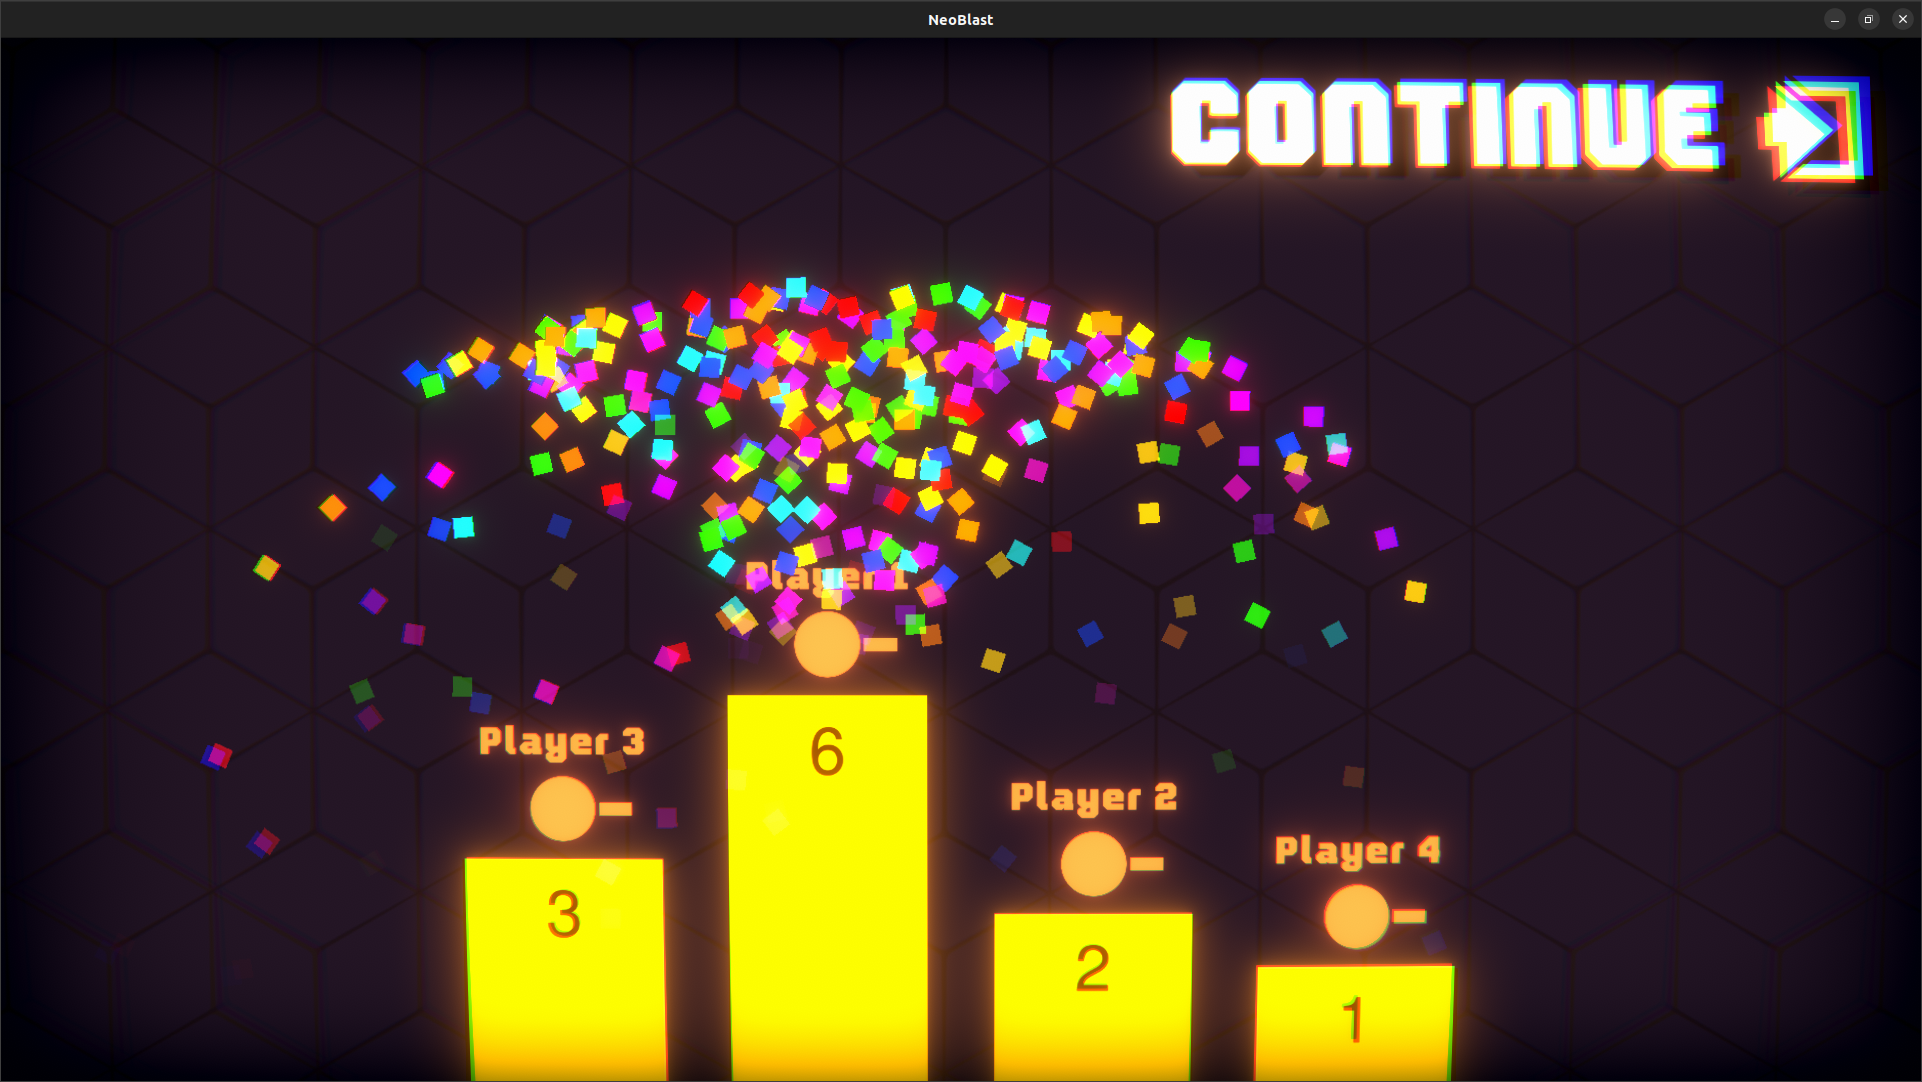
\includegraphics[width=0.9\textwidth, height = 4cm]{images/game/podium.png}
        \caption{Podium}
        \label{fig:podium}
    \end{subfigure}
\end{figure}

\section{Structure}
Ce projet peut être séparé en deux parties : une partie matérielle (hardware) et une partie logicielle (software). En raison de problèmes d’approvisionnement qui ont suivi la récente pandémie et suite à la complexité inattendue de la partie logicielle, la partie matérielle a été moins développée que ce que nous souhaitions.

\subsection{Partie matérielle (Hardware)}
Cette partie consiste en une Raspberry Pi 3 modèle B+ avec une carte microSD, d’un petit câble et d’une batterie portable de 5000 mAh fournissant 5 V à 2.1 A. La Raspberry provient d’une connaissance de Fabio, qui a gracieusement accepté de nous la prêter pour notre projet.
La figure \ref{fig:images_raspberry} montre deux photos de la Raspberry Pi et deux photos du dispositif complet.

\begin{figure}
    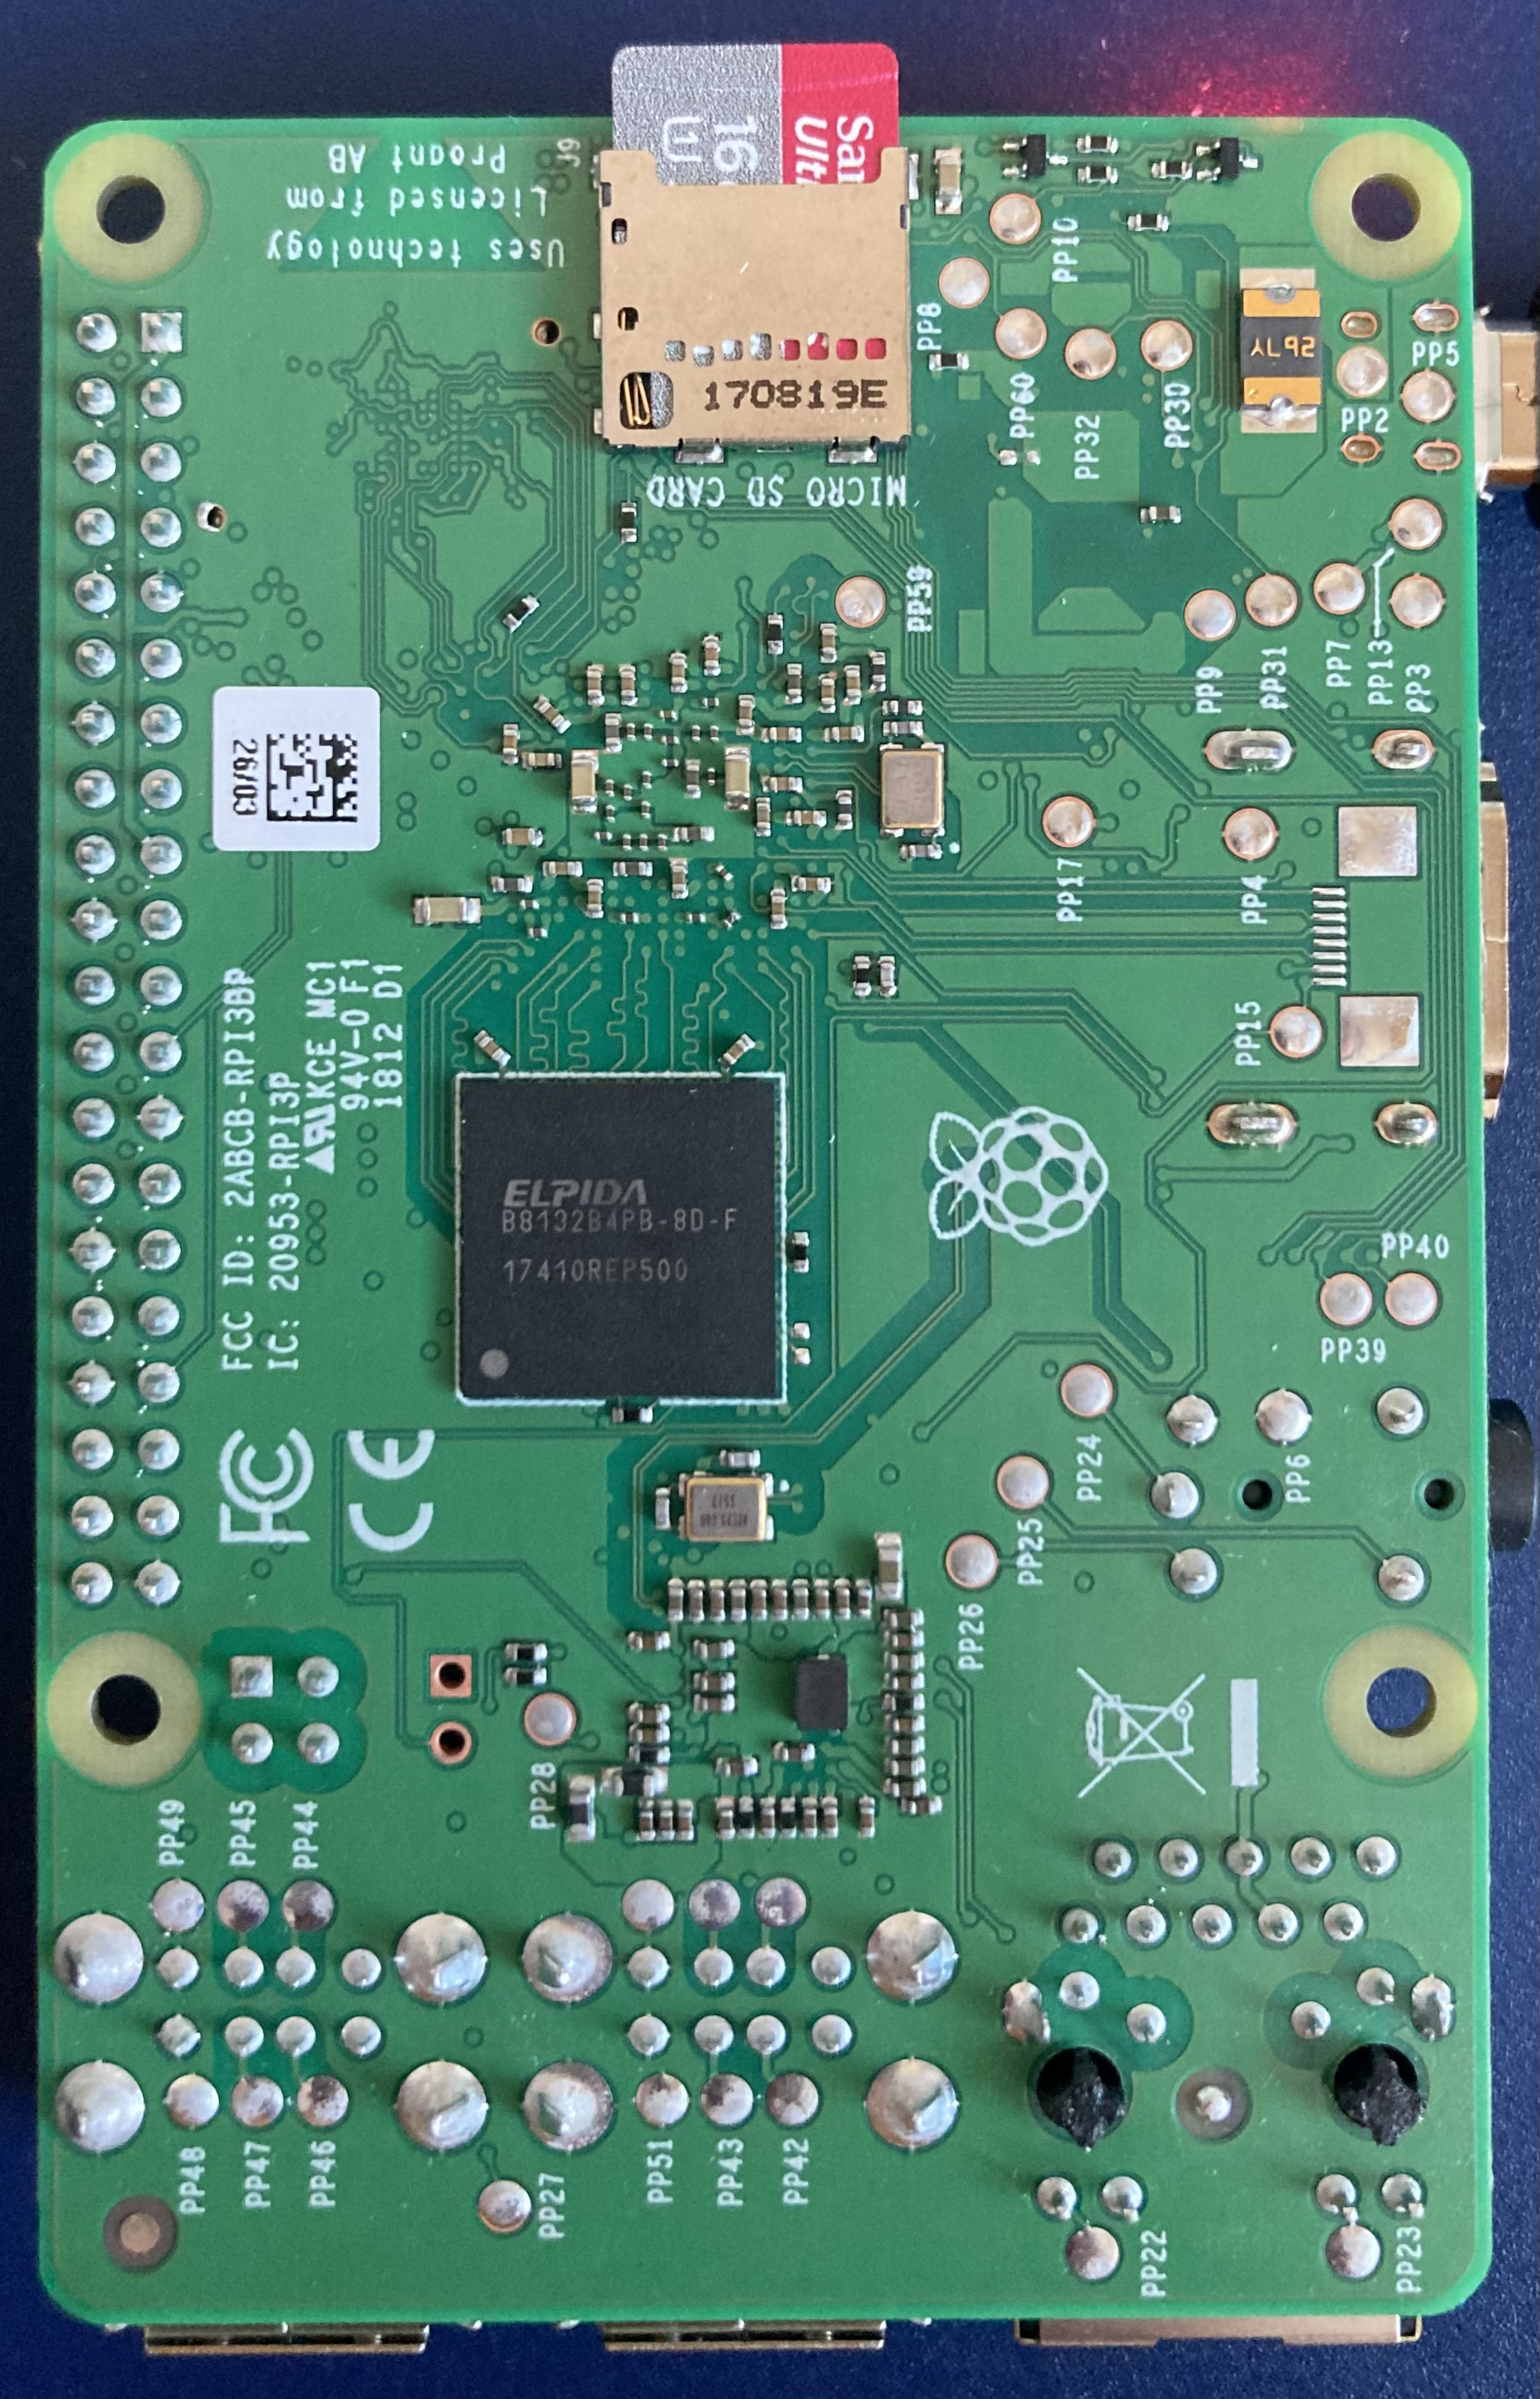
\includegraphics[width=0.5\textwidth, height = 12cm]{images/hardware/Raspberry3.jpg}
    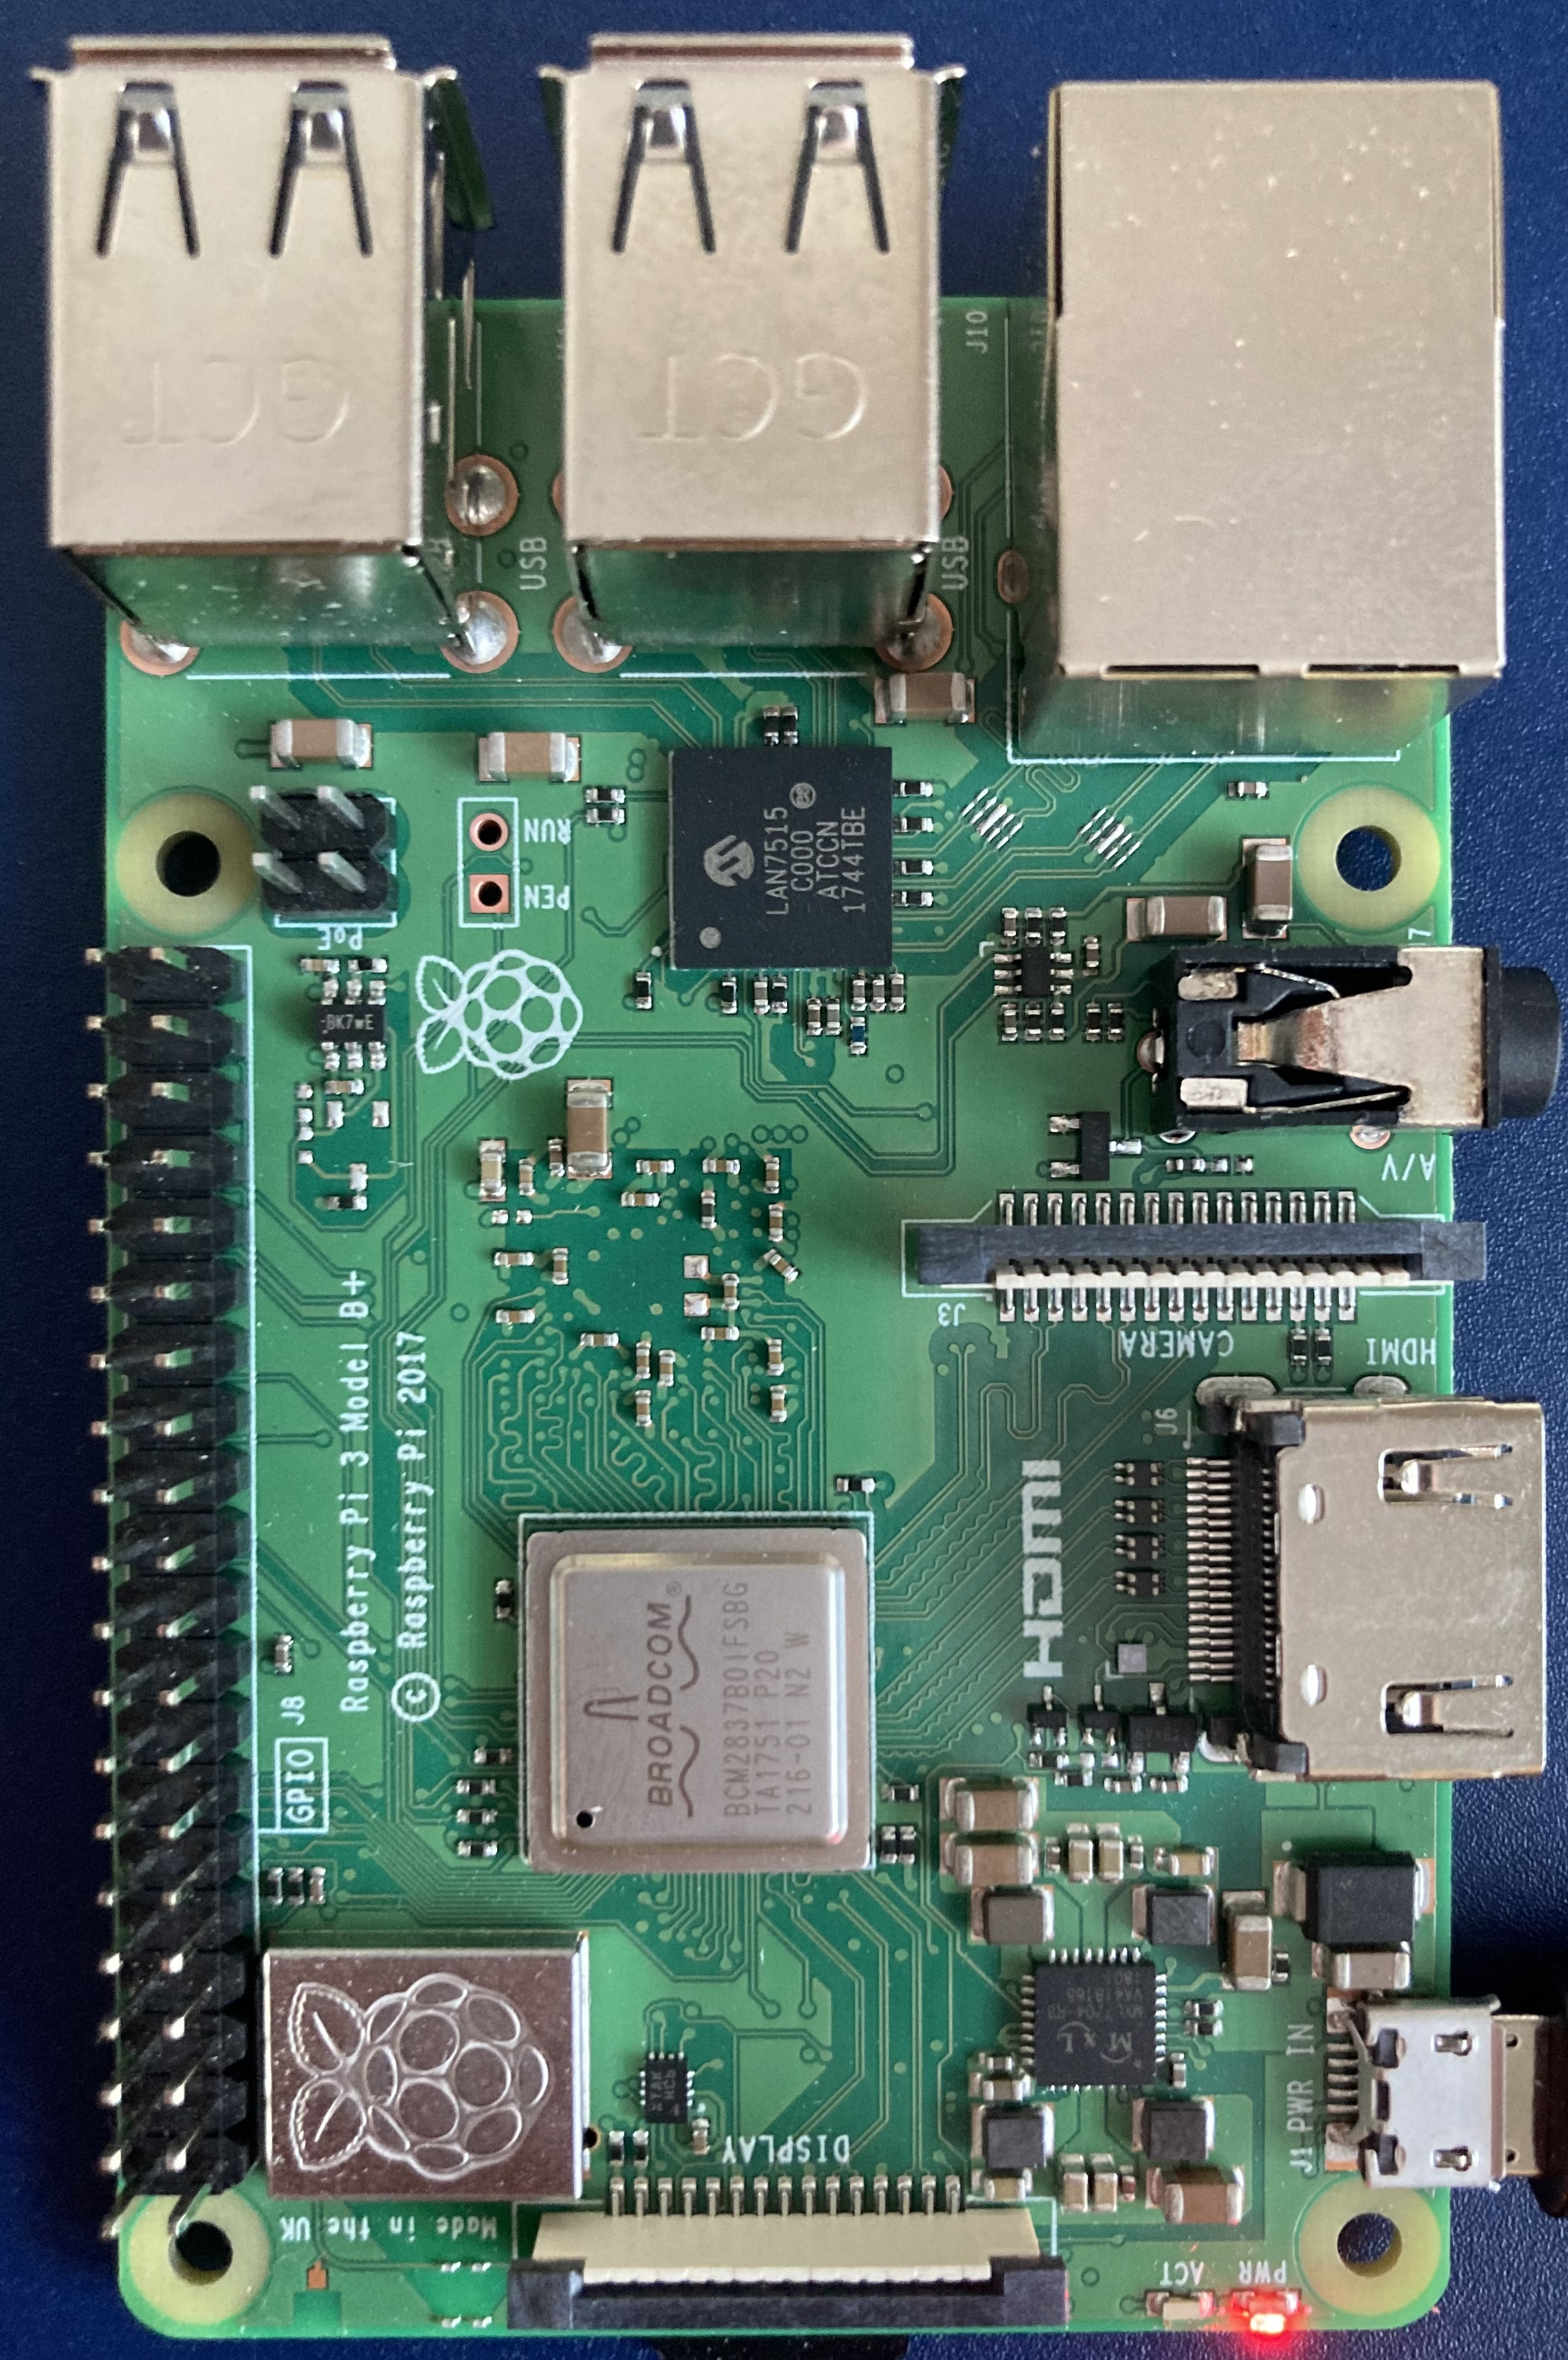
\includegraphics[width=0.5\textwidth, height = 12cm]{images/hardware/Raspberry2.jpg}
    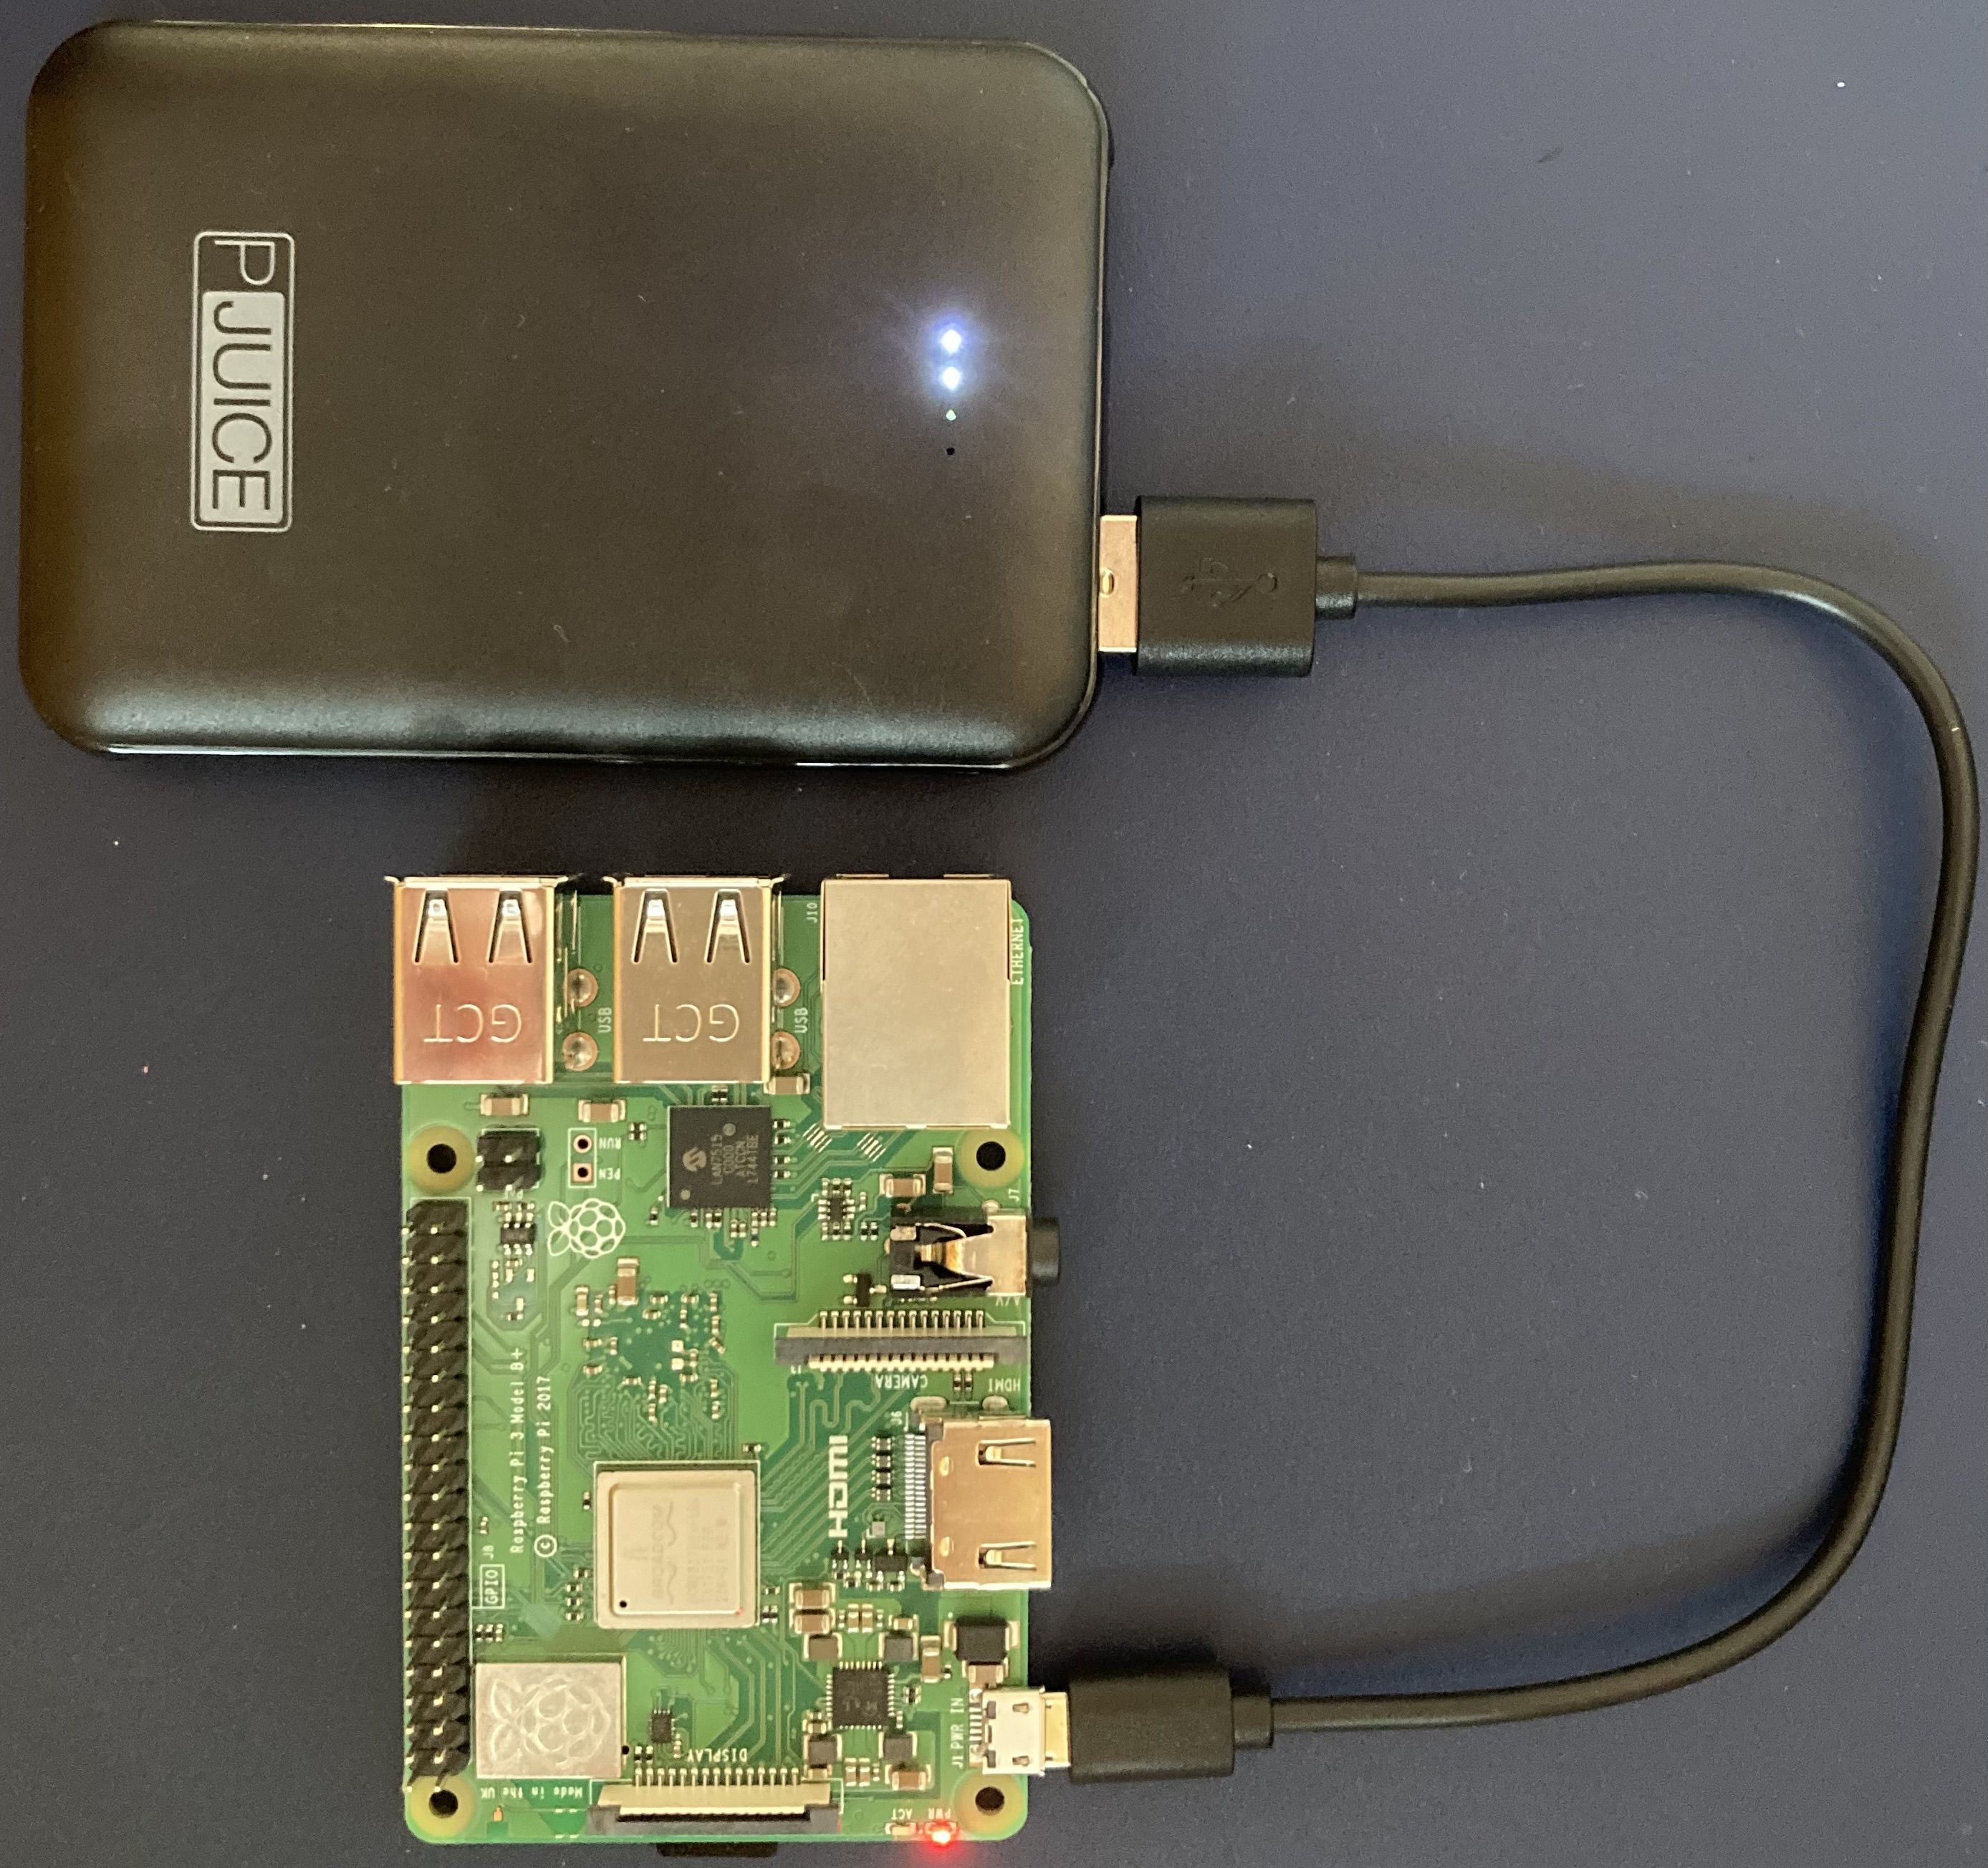
\includegraphics[width=0.5\textwidth, height = 6cm]{images/hardware/Raspberry1.jpg}
    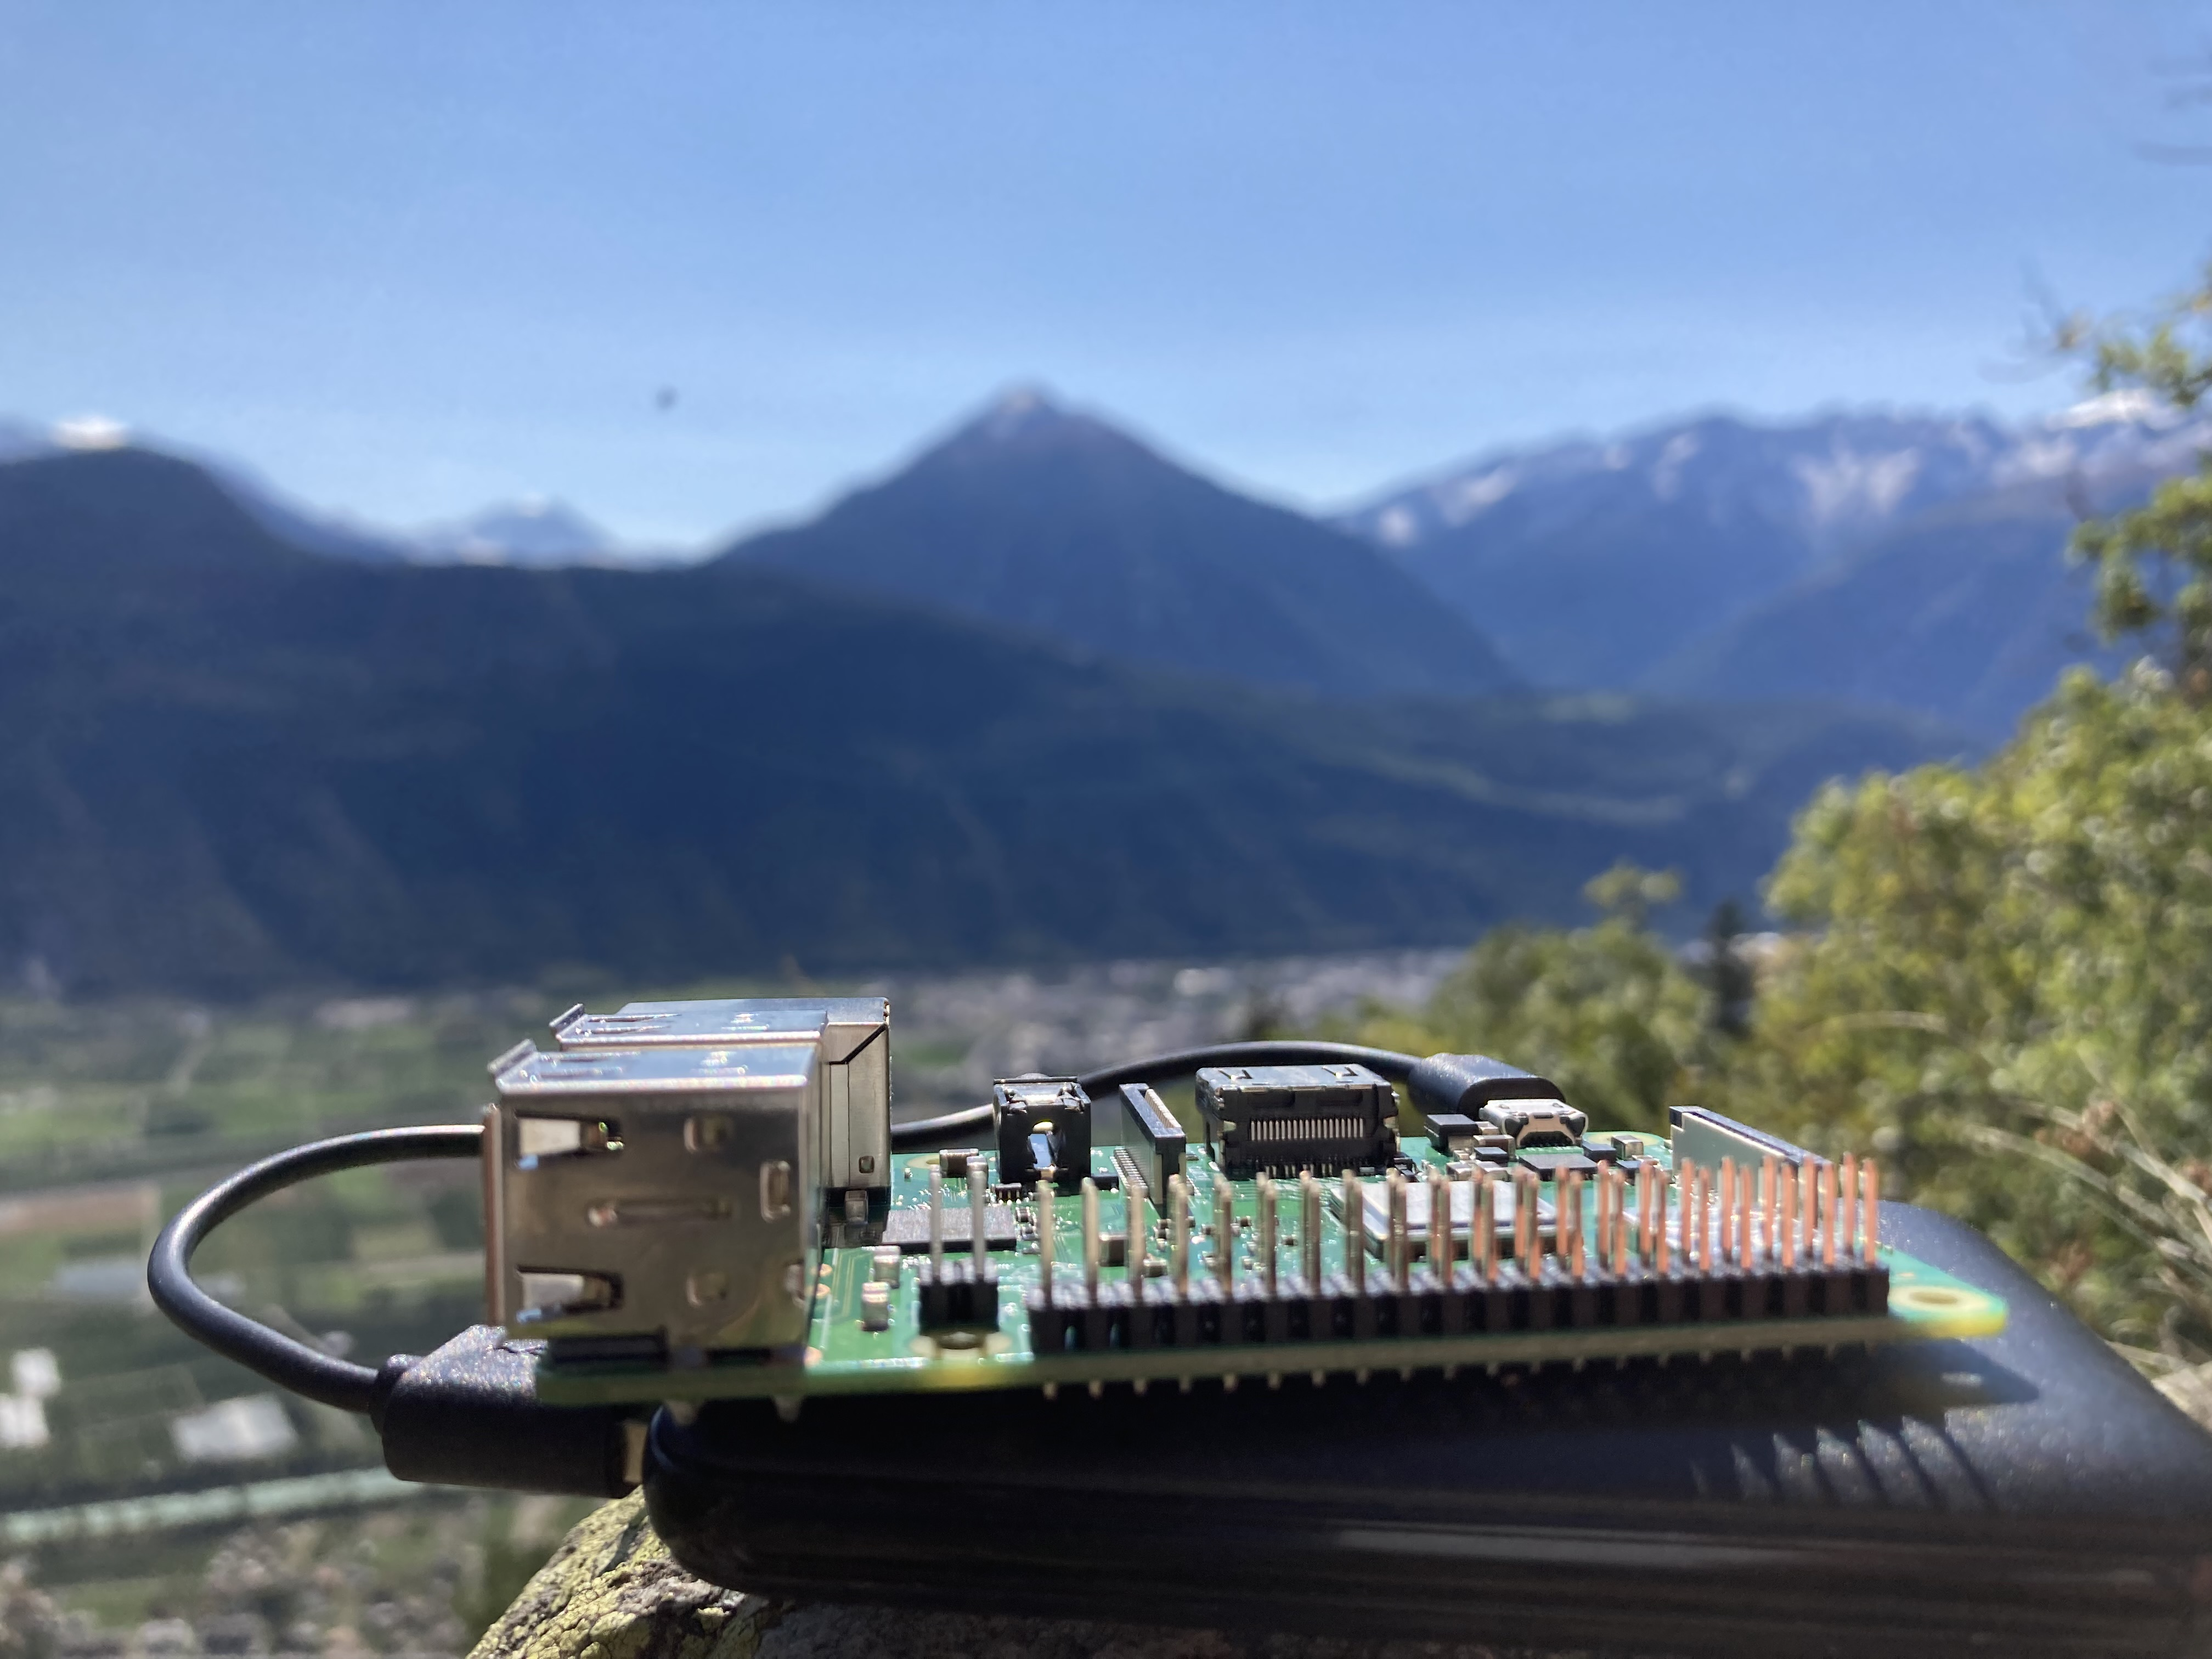
\includegraphics[width=0.5\textwidth, height = 6cm]{images/hardware/Raspberry4.jpg}
    \caption{Images du dispositif}
    \label{fig:images_raspberry}
\end{figure}

\subsection{Partie logicielle (Software)}
La partie logicielle est constituée du code nécessaire au fonctionnement du jeu. Afin de conserver un historique des versions ainsi que pour pouvoir collaborer, nous avons utilisé le programme Git \cite{git}.
Notre projet est hébergé à cette adresse : \url{https://github.com/DanielRoulin/Waypoint} \\
Le plus simple pour étudier le projet consiste à télécharger le code source avec la commande suivante:
\begin{minted}{bash}
git clone https://github.com/DanielRoulin/Waypoint.git
\end{minted}
Un dossier nommé \emph{Waypoint} contenant le code source sera normalement créé. \\
Waypoint est le nom que nous avons donné à ce projet, NeoBlast est le nom du jeu et Theel est le nom d'utilisateur de Fabio sur GitHub. \\
Voici une vue d’ensemble du projet:
\begin{minted}{text}
~/Waypoint$ tree -a -L 1
Waypoint
├── Client
├── Server
├── Design
├── Statistics
├── Rapport
├── LICENSE
├── README.md
└── .git
 
4 directories
\end{minted}

\noindent Tout d’abord, nous avons les deux dossiers les plus importants : \emph{Client} et  \emph{Server}. C’est là que se situe la plus grande partie de notre travail, séparée entre le code exécuté sur le client (téléphone ou ordinateur) et le code exécuté sur le serveur (Raspberry Pi ou VPS \cite{vps}). Le dossier \emph{Rapport} contient ce PDF ainsi que le document \LaTeX\ utilisé pour le créer. Ensuite, le dossier \emph{Design} contient nos réflexions concernant la conception du boîtier et un logo, tandis que le dossier \emph{.git} stocke toutes les informations nécessaires au contrôle de version. Le dossier \emph{Statistics} contient les scripts générant les graphiques de la section \ref{section:chiffres}. Le fichier \emph{LICENSE} contient la licence de ce projet. Nous avons choisi la \textit{GNU General Public License v3.0}\footnote{\url{https://www.gnu.org/licenses/gpl-3.0.en.html}}, qui autorise l'utilisation commerciale, la modification et la distribution de notre code, à condition que nous soyons cité et que le projet utilise la même licence. Finalement, le fichier \emph{README.md} contient un très court résumé du projet.

\subsubsection{Serveur}
Ce dossier a la structure d’une application \textit{.NET} classique. Il est donc nécessaire d'installer ce programme pour compiler notre projet. 
Pour installer \textit{.NET} sur Ubuntu, par exemple, il suffit d'exécuter cette commande:
\begin{minted}{text}
sudo apt-get update && sudo apt-get install -y dotnet6
\end{minted}
Des instructions plus détaillées sont disponibles à cette adresse: \\
\url{https://learn.microsoft.com/en-us/dotnet/core/install/linux} \\
\\
Pour lancer le projet, le plus simple consiste à l'ouvrir avec l'éditeur \textit{VSCode}, car le dossier \mbox{\emph{.vscode}} contient la configuration nécessaire. Sinon, pour simplement lancer le projet, il faut exécuter la commande suivante dans le dossier \emph{Server}:
\begin{minted}{text}
dotnet run
\end{minted}
Et pour compiler le projet pour Linux (toujours dans le dossier \emph{Server}):
\begin{minted}{text}
build GameServer.csproj -r linux-x64 -o bin/Linux/
\end{minted}
ou pour compiler le projet pour la Raspberry Pi:
\begin{minted}{text}
build GameServer.csproj -r linux-arm -o bin/Raspberry/
\end{minted}
Après avoir compilé le projet, il ne faut pas oublier de copier le dossier \emph{Scenes} là où il est exécuté.\\
\\
Note : Si le message suivant apparaît, c'est parce que nous utilisons une version dépassée de \textit{.NET}, car le tutoriel que nous avons suivi utilise cette dernière, et que \textit{.NET} est rétrocompatible. (voir la section \ref{section:demarche} pour plus de détails)
\begin{minted}{text}
warning NETSDK1138: The target framework 'netcoreapp3.0' is out of support and will not receive security updates in the future.
\end{minted}
Voici les différents fichiers du serveur :
\begin{minted}{text}
tree -a --dirsfirst Server
Server/
├── .vscode
│   ├── launch.json
│   ├── settings.json
│   └── tasks.json
├── bin
│   ├── Debug
│   │   └── ...
│   ├── Linux
│   │   └── ...
│   └── Raspberry
│       └── ...
├── Scenes
│   ├── Maps
│   │   ├── Map1.unity
│   │   ├── Map2.unity
│   │   ├── Map3.unity
│   │   ├── Map4.unity
│   │   └── Map5.unity
│   └── WaitingRoom.unity
├── GameServer.csproj
├── .gitignore
├── Client.cs
├── Colliders.cs
├── Constants.cs
├── GameLogic.cs
├── Item.cs
├── Packet.cs
├── Player.cs
├── Program.cs
├── Projectile.cs
├── Scene.cs
├── Server.cs
├── ServerHandle.cs
├── ServerSend.cs
├── ThreadManager.cs
└── Utilities.cs 

22 directories, 753 files
\end{minted}
\begin{itemize}
    \item Le dossier \emph{.vscode} contient la configuration de notre éditeur:\emph{VSCode}.
    \item Le fichier \emph{tasks.json} contient les instructions pour compiler le projet.
    \item Le fichier \emph{launch.json} contient celle pour le déboguer.
    \item Le fichier \emph{settings.json} contient nos différents réglages de l'éditeur.
    \item Le dossier \emph{bin}, qui n’est pas inclus sur github, contient tous nos builds \cite{build} pour les différentes plateformes, en l'occurrence Linux et Raspberry.
    \item Le dossier \emph{obj} est créé lors de la compilation et contient les fichiers créés pendant l'étape intermédiaire entre la compilation et le linting.
    \item Le dossier \emph{Scenes}, qui contient une copie des terrains du client, au format .unity. Ce format s’appelle UnityYAML \cite{unityyaml} et, comme son nom l’indique, il s'agit du format des scènes Unity, basé sur le format YAML. Il contient la salle d’attente, \emph{WaitingRoom.unity} et toutes les cartes du jeu : \emph{Map1.unity}, \emph{Map2.unity}, ...
    \item \emph{GameServer.csproj} contient les réglages du projet. En voici une copie :
    \begin{minted}{xml}
<Project Sdk="Microsoft.NET.Sdk">
 <PropertyGroup>
   <OutputType>Exe</OutputType>
   <TargetFramework>netcoreapp3.0</TargetFramework>
   <RollForward>Major</RollForward>
 </PropertyGroup>
 <ItemGroup>
   <PackageReference Include="System.Numerics.Vectors" Version="4.5.0" />
   <PackageReference Include="YamlDotNet" Version="11.2.1" />
 </ItemGroup>
</Project>
    \end{minted}
    On peut voir que l’on demande au compilateur de créer un fichier exécutable, en utilisant la version 3.0 de \textit{.NET} si possible mais en acceptant n’importe quelle version au-dessus. De plus, nous importons le package \emph{System.Numerics.Vectors}, qui nous permet d’utiliser des vecteurs ainsi que le package \emph{YamlDotNet} \cite{yamldotnet} qui nous permet de parser \cite{parser} du \textit{YAML}.
    
    \item \emph{.gitignore} contient une liste des fichiers ou dossiers que Git \cite{git} doit ignorer. En l'occurrence, on ne souhaite ignorer que les résultat de la compilation:
    \begin{minted}{text}
bin
obj
    \end{minted}
\end{itemize}
Les fichiers restants sont les scripts, qui sont le cœur du serveur. Voici un tableau résumant leurs fonctions respectives :
\begin{center}
\begin{longtable}{|l|p{10cm}|}
    \hline
    Fichier & Fonction \\
    \hline\hline
    \mintinline{text}{Program.cs}\footnotemark[1] & Premier script appelé lors de l’exécution, \emph{Program.cs} est responsable du démarrage du serveur et de la \textit{game loop} dans deux différents \textit{threads}. Il actualise le jeu à intervalles réguliers.\\
    \hline
    \mintinline{text}{ThreadManager.cs}\footnotemark[1] & Ce script gère simplement la communication entre le \textit{thread} du serveur et la \textit{game loop} (\textit{main thread}).\\
    \hline
    \mintinline{text}{Server.cs}\footnotemark[1] & \emph{Server.cs} contient la classe la plus importante du projet, la classe \emph{Server}. Cette classe stocke toutes les informations de la partie, telle que sa durée, la liste des joueurs, des objets et des projectiles, etc. Elle est responsable de l’initialisation du serveur et de la connexion des nouveaux joueurs.\\
    \hline
    \mintinline{text}{Client.cs}\footnotemark[1] & Ce fichier contient la classe \emph{Client}, qui est instancié pour chaque joueur connecté. Cependant, elle n’est responsable que de la gestion de la connexion, les fonctions liées au joueur se situent dans la classe \emph{Player}. Chaque \emph{Client} a un \emph{Player} associé et est chargé de l'initialiser et de le réinitialiser quand le client se déconnecte.\\
    \hline
    \mintinline{text}{Packet.cs}\footnotemark[1] & Cette classe contient la logique nécessaire à l’encodage et au décodage des paquets, qui sont formés d’octets. Il contient aussi la liste et le nom des différents paquets, qui doit impérativement être la même sur le client et le serveur.\\
    \hline
    \mintinline{text}{ServerSend.cs} & Cette classe contient les fonctions responsables de la construction et de l’encodage des paquets envoyés par le serveur aux clients.\\
    \hline
    \mintinline{text}{ServerHandle.cs} & Cette classe contient les fonctions responsables du décodage et de l'interprétation des paquets envoyés par les clients au serveur.\\
    \hline
    \mintinline{text}{GameLogic.cs} & C’est ici que se situe la logique du jeu. Ce script contient la fonction \emph{Update}, qui est appelée à chaque tic et s’occupe de mettre à jour les joueurs, les projectiles et les objets, ainsi que les fonctions permettant de démarrer et d'arrêter le jeu.\\
    \hline
    \mintinline{text}{Scene.cs} & Ce fichier est responsable de l’interprétation des scènes, qui se situe dans le dossier \emph{Scenes}. Il est responsable de trouver certains objets dans les scènes, tel que les obstacles, les éléments déclencheur d’action (\textit{trigger}) ainsi que les points d’apparition (\textit{spawn points}).\\
    \hline
    \mintinline{text}{Player.cs} & Cette classe est instanciée pour chaque joueur, et contient toutes leurs informations, telles que leur position, leur rotation, leur nom, leur armes, etc. Elle est aussi responsable de leurs interactions, telles que récupérer des armes ou tirer des projectiles.\\
    \hline
    \mintinline{text}{Item.cs} & Cette classe est instanciée pour chaque objet du jeu, et contient toutes leurs informations, telles que leur position et type.\\
    \hline
    \mintinline{text}{Projectile.cs} & Cette classe est instanciée pour chaque projectile du jeu, et contient toutes leurs informations, telles que leur position, rotation et type. Elle est aussi responsable de changer leur position, en suivant différentes trajectoires en fonction de leur type.\\
    \hline
    \mintinline{text}{Collider.cs} & Ce fichier est responsable de détecter les collisions du jeu. Il contient deux classes: \emph{RectCollider} et \emph{CircleCollider}, représentant respectivement des rectangles et des cercles. Chaque entité du jeu possède un de ces \textit{collider}. Chacune des classes contient une fonction permettant de vérifier qu'elle n’intersecte pas avec un autre collider.\\
    \hline
    \mintinline{text}{Utilities.cs} & Cette classe contient diverses fonctions pratiques, liées notamment à la génération de nombres aléatoires, de position aléatoire spécifiques et au logging\\
    \hline
    \mintinline{text}{Constants.cs} & Cette classe contient toutes les constantes du jeu, telles que le nombre de tic par seconde, la taille des terrains, les caractéristiques des différentes armes et les noms par défaut des joueurs.\\ 
    \hline
\end{longtable}
\end{center}
\hrule
\textit{\footnotemark[1]Nous n’avons que très peu modifié ces fichiers, ils proviennent du tutoriel de Tom Weiland. Voir la section \ref{section:demarche}.}

\subsubsection{Client}
Le deuxième grand dossier de ce projet est le dossier \emph{Client}. Ce dernier contient l'entièreté du code source du client, qui est un projet Unity. Le lien ci-dessous explique comment installer la plateforme, ce qui est nécessaire pour ouvrir et compiler le projet: \\
\url{https://unity3d.com/get-unity/download} \\
Notre projet utilise la version 2020.3.2f1, mais fonctionne sur d'autres versions supérieures.
En voici une vue d'ensemble:
\begin{minted}{text}
tree -a --dirsfirst Client
Client
├── Assets
│   ├── Animations
│   │   └── ...
│   ├── Fonts
│   │   └── ...
│   ├── Graphic
│   │   └── ...
│   ├── _Heathen Engineering
│   │   └── ...
│   ├── Hexanim
│   │   └── ...
│   ├── Materials
│   │   └── ...
│   ├── Prefabs
│   │   └── ...
│   ├── Scenes
│   │   ├── Maps
│   │   │   ├── Map1.unity
│   │   │   ├── Map2.unity
│   │   │   ├── Map3.unity
│   │   │   ├── Map4.unity
│   │   │   └── Map5.unity
│   │   ├── Empty.unity
│   │   ├── End Screen.unity
│   │   └── WaitingRoom.unity
│   ├── Scripts
│   │   ├── CameraSC.cs
│   │   ├── Client.cs
│   │   ├── ClientHandle.cs
│   │   ├── ClientSend.cs
│   │   ├── DontDestroy.cs
│   │   ├── EndScreenBar.cs
│   │   ├── EndScreenManager.cs
│   │   ├── GameManager.cs
│   │   ├── Item.cs
│   │   ├── Leaderboard.cs
│   │   ├── LeaderboardEntry.cs
│   │   ├── Menu.cs
│   │   ├── Packet.cs
│   │   ├── PlayerController.cs
│   │   ├── PlayerManager.cs
│   │   ├── Projectile.cs
│   │   └── ThreadManager.cs
├── ProjectSettings
│   └── ...
├── UserSettings
│   └── EditorUserSettings.asset
├── .vscode
│   └── settings.json
└── .gitignore
 
55 directories, 1635 files
\end{minted}
\hrule
\textit{Note: Les fichiers .meta ne sont pas affichés. Ils sont créés par Unity et ne contiennent que des métadonnées concernant les fichiers du même nom.} \\
\begin{itemize}
\item Le dossier \emph{.vscode} contient, comme sur le serveur, la configuration de notre éditeur.
\item Le fichier \emph{settings.json} contient  une liste de fichier à ne pas montrer dans l’éditeur afin de simplifier l’affichage.
\item Les dossiers \emph{ProjectSettings} et \emph{UserSettings} contiennent respectivement les réglages du projet et ceux de l’utilisateur.
\item Les dossiers \emph{Animations}, \emph{Fonts} et \emph{Materials} contiennent des animations, des polices d’écriture ainsi que des matériaux (texture). 
\item Le dossier \emph{Prefab} contient tous les \textit{prefabs} du projet. Un \textit{prefab}, dans Unity, est un objet pouvant être instancié plusieurs fois dans une scène. Par exemple, les joueurs et les projectiles sont des \textit{prefabs}.
\item Le dossier \emph{Scenes} contient tous les terrains du jeu et doit être exactement le même que sur le serveur.
\item Le dossier \emph{Scripts} contient tous les scripts du projet.
\end{itemize}
Voici un tableau résumant leurs fonctions respectives:
\begin{center}
\begin{longtable}{|l|p{10cm}|}
    \hline
    Fichier & Fonction \\
    \hline\hline
    \mintinline{bash}{ThreadManager.cs}\footnotemark[1] & Ce script gère simplement la communication entre le \textit{thread} du client et la \textit{game loop} (\textit{main thread}).\\
    \hline
    \mintinline{bash}{Client.cs}\footnotemark[1] & Cette classe est responsable de la connexion avec le serveur. Elle gère le transfert de paquets via TCP et UDP.\\
    \hline
    \mintinline{bash}{Packet.cs}\footnotemark[1] & Ce fichier est le même que sur le serveur.\\
    \hline
    \mintinline{bash}{ClientSend.cs} & Cette classe contient les fonctions responsables de la construction et de l’encodage des paquets envoyés par le client au serveur, tels que les boutons qu’il presse, sa rotation ou son nom d’utilisateur.\\
    \hline
    \mintinline{bash}{ClientHandle.cs} & Cette classe contient les fonctions responsables du décodage et de l'interprétation des paquets envoyés par le serveur au client, tel que la position des autres entitées ou le nom des autres joueurs.\\
    \hline
    \mintinline{bash}{GameManager.cs} & Cette classe est la plus importante du client, car elle est responsable du déroulement du jeu. Par exemple, elle s’occupe de charger les différentes cartes, de démarrer et terminer les parties et de faire apparaître les joueurs, les projectiles et les objets sur la scène.\\
    \hline
    \mintinline{bash}{Menu.cs} & Cette classe gère tous les menus (UI) du jeu.\\
    \hline
    \mintinline{bash}{PlayerManager.cs} & Cette classe est associée à chaque joueur apparaissant sur la scène et est responsable de leur apparence et comportement.\\
    \hline
    \mintinline{bash}{PlayerController.cs} & Cette classe s’occupe d'envoyer au serveur le nom du joueur local ainsi que les différents boutons qu’il presse.\\
    \hline
    \mintinline{bash}{Item.cs} & Cette classe est instanciée pour chaque objet du jeu, et contient toutes leurs informations, telles que leur position et type.\\
    \hline
    \mintinline{bash}{Projectile.cs} & Cette classe est associée à chaque projectile et s’occupe de les déplacer et de les détruire.\\
    \hline
    \mintinline{bash}{CameraSC.cs} & Ce script est rattaché à la caméra et est responsable de son mouvement, pour qu’elle suive le joueur de façon fluide.\\
    \hline
    \mintinline{bash}{Leaderboard.cs} & Cette classe gère le tableau des scores qui apparaît en haut à droite durant une partie. Il se charge notamment de trier les joueurs par leurs scores.\\
    \hline
    \mintinline{bash}{LeaderboardEntry.cs} & Cette classe est associée à chaque entrée du tableau des scores, stocke leur position et leur texte, et est responsable de l’animation de leur position.\\
    \hline
    \mintinline{bash}{EnsScreenManager.cs} & Ce fichier contient la classe responsable de l’écran apparaissant à la fin d’une partie\\
    \hline
    \mintinline{bash}{EndScreenBar.cs} & Cette classe est responsable du podium qui apparaît à la fin de la partie.\\
    \hline
    \mintinline{bash}{DontDestroy.cs} & Ce script est très petit et ne fait qu'indiquer au compilateur de ne pas détruire certains éléments quand une nouvelle carte est chargée.\\
    \hline
\end{longtable}
\end{center}
\hrule
\textit{\footnotemark[1]Nous n’avons que très peu modifié ces fichiers, ils proviennent du tutoriel de Tom Weiland. Voir la section \ref{section:demarche}.}

\subsection{Protocole}
Pour communiquer entre eux, le client et le serveur utilisent deux protocoles de base: TCP \cite{tcp} et
UDP \cite{udp}. Ils transfèrent des séquences d’octets, appelées paquets (\textit{packets}). La signification d’un paquet dépend de son \mintinline{text}{packetId} mais aussi de l’état du client qui le reçoit. Par défaut, le port 26950 est utilisé. \\
Voici une vue d’ensemble du format d’un paquet:
\begin{center}
\begin{tabular}{|l|l|p{10cm}|}
    \hline
    Nom & Type & Notes \\
    \hline\hline
    \mintinline{text}{length} & int & Longueur du message. Est égal à la longueur du \mintinline{text}{packetId} + la longueur des donnée du packet. \\
    \hline
    \mintinline{text}{packetId} & int & Type du paquet, voir les sections suivantes. \\
    \hline
    \mintinline{text}{data} & bytes & Liste d’octets dépendant du \mintinline{text}{packetId}. \\
    \hline
\end{tabular}
\end{center}
Le même format est utilisé si la connexion est en TCP ou en UDP.

\subsubsection{TCP OU UDP ?}
Le jeu utilise deux types de connexion: TCP et UDP. TCP à l’avantage de garantir l'arrivée d’un paquet si un client peut le recevoir, ainsi que de conserver l’ordre des paquets. UDP est plus rapide que TCP, mais ne vérifie pas la réception ni l’ordre des paquets. C’est pourquoi TCP est privilégié pour les messages importants, envoyés qu'une seule fois, tandis qu’UDP est utilisé pour les messages envoyés à chaque tic. En pratique, seul le temps, la position et la rotation utilisent UDP. Un autre inconvénient d’UDP est que certains réseaux, notamment celui de notre collège, semblent bloquer ce protocole. C’est pourquoi nous aurions souhaité ajouter à notre jeu un mode “TCP only”, ce que nous n'avons malheureusement pas eu le temps de faire.

\subsubsection{Le client (n’) est (pas) roi}
Lorsque l’on développe un jeu en ligne, il est nécessaire de choisir la liberté du client. Par exemple, le client pourrait simplement envoyer sa position sous forme de vecteur au serveur. Cependant, cela implique au serveur de faire confiance au client pour qu’il n’envoie pas des positions interdites ou erronées, car ce dernier pourrait ainsi se téléporter. C’est pourquoi notre jeu, comme la plupart des jeux en ligne, demande au client d’uniquement envoyer ses clics de boutons, puis le serveur envoie la position du joueur comme celle de n’importe quelle autre joueur, sous forme de vecteur. De plus, si plusieurs paquets de mouvement sont envoyés en un seul tic, le serveur n’applique que le dernier reçu. Cela permet de contrôler la vitesse des joueurs. La seule exception à cette règle est la rotation du joueur, que le client contrôle entièrement afin d’éviter un délai nettement visible.

\subsubsection{Types de données}
Voici un tableau résumant les 6 types de données utilisé par le protocole:
\begin{center}
\begin{tabular}{|l|m{1.5cm}|m{5cm}|m{5cm}|}
    \hline
    Nom & Taille (octets) & Encode & Notes \\
    \hline\hline
    byte & 1 & Un octet, nombre entier entre 0 et 255 & Unsigned 8-bit integer \\
    \hline
    int & 4 & Un nombre entier entre \mbox{-2147483648} et 2147483647  & Signed 32-bit integer, two's complement \\
    \hline
    float & 4 & Un nombre à virgule flottante & A single-precision 32-bit IEEE 754 floating point number \\
    \hline
    bool & 1 & Vrai ou faux & True is encoded as 0x01, false as 0x00. \\
    \hline
    string (n) & 4 + n & Une séquence de caractère du tableau ASCII (7 bits) & ASCII (7 bits) string prefixed with its size in bytes as an int \\
    \hline
    vector2 & 2 * 4 & Un vecteur 2 dimensionnel & X as a float, followed by Y as a float \\
    \hline
\end{tabular}
\end{center}
Ces représentations proviennent simplement de la fonction \mintinline{csharp}{BitConverter.GetBytes} du \textit{namespace} \cite{namespace} \mintinline{csharp}{System}. \\
Une liste détaillée des paquet se situe dans l'annexe \ref{annexe:paquets}.

\section{Quelques chiffres}
\label{section:chiffres}
\subsection{Lignes de code en fonction du temps}
\begin{figure}[h]
    \centering
    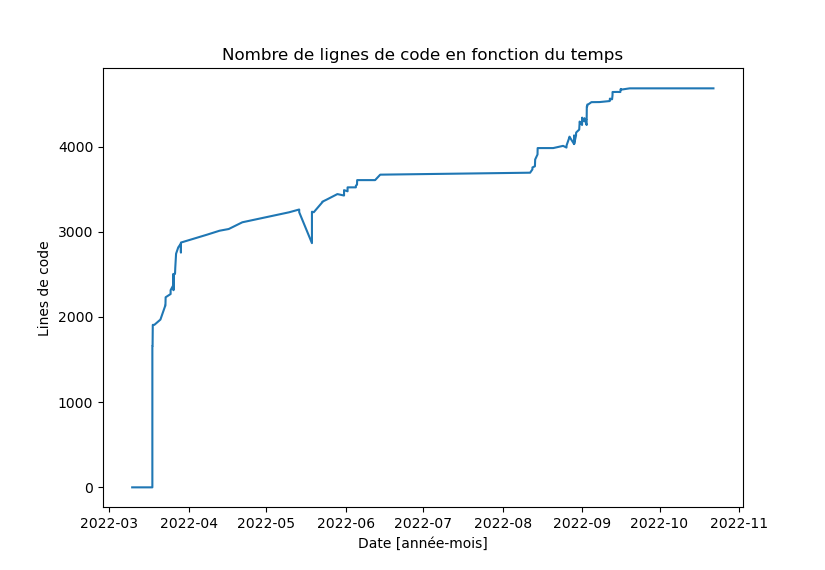
\includegraphics[width=0.8\textwidth]{images/stats/lines_of_code.png}
    \caption{Lignes de code en fonction du temps}
    \label{fig:lines_of_code}
\end{figure}
\noindent Le graphique \ref{fig:lines_of_code} montre le nombre de lignes contenu dans les fichiers .cs (fichiers de code C\#) en fonction du temps. Il a pu être fait en remontant dans l’historique des versions via Git. On constate la réorganisation du projet mi-mars 2022, suivi de l’ajout du code du tutoriel, puis l’adaptation du projet à nos besoins en fin du mois de mars. Les changements brutaux sont dus à des conflits de fusion de notre code (\textit{merge conflicts}) qui ont été résolus avec plus ou moins de succès. La grosse vallée fin mai représente un changement de nos menus (UI), d'où la suppression et l’ajout rapide de code. On peut aussi voir une période de calme pendant les vacances, de juin à fin août. L’agitation à la fin du mois de mai correspond de nouveau à des conflits de fusion, car nous travaillions en même temps aux mêmes endroits. Finalement, les changements du mois d’octobre représentent notre débogage, c’est pourquoi peu d’ajouts de code peuvent être observés.

\newpage
\subsection{Contributions}

\begin{figure}[h]
    \begin{subfigure}{0.5\textwidth}
        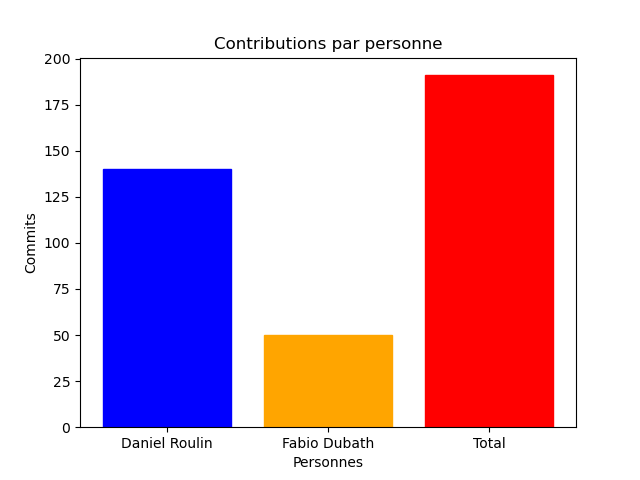
\includegraphics[width=0.9\textwidth]{images/stats/contributions.png}
        \centering
        \caption{Contributions}
        \label{fig:contributions}
    \end{subfigure}
        \begin{subfigure}{0.5\textwidth}
        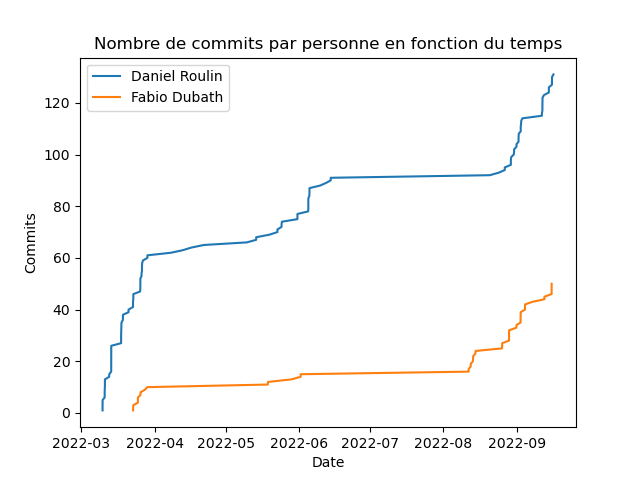
\includegraphics[width=0.9\textwidth]{images/stats/commits.png}
        \centering
        \caption{Commits}
        \label{fig:commits}
    \end{subfigure}
\end{figure}

\noindent Le graphique \ref{fig:contributions} montre le nombre de \textit{commits} par personne. À première vue, on pourrait penser que Fabio a moins contribué aux projets. Cependant, les commits ne sont pas représentatifs du travail total fourni. En effet, nous avons tous les deux différentes façons de contribuer. Par exemple, Daniel préfère créer un \textit{commit} à chaque changement, tandis que Fabio le fait quand il a fini toute une partie. De plus, Fabio s’est aussi concentré sur la partie artistique, qui n’est pas mesurée par les commits.\\

\noindent Le graphique \ref{fig:commits} montre  l'évolution du nombre de \textit{commits} en fonction du temps. On y voit nos deux différents styles, ainsi que les différentes périodes du projet. Le décalage entre les deux courbes est aussi dû au fait que le \textit{repo} était à l’origine utilisé uniquement pour le serveur, avant d’avoir fusionné avec le reste du projet (voir la section \ref{section:demarche}). C’est pourquoi les premiers \textit{commits} ont été faits seulement par Daniel et commencent plus tôt.



\section{Démarche}
\label{section:demarche}
Ce chapitre parle du processus de création du projet, de la première idée au produit fini. 
\subsection{L’idée}
Tout a commencé en cours de philo, durant une phase soudaine d'ennui profond. Nous nous sommes mis à discuter. C'est là que nous avons réalisé qu'il n’était alors pas possible de jouer à des jeux en ligne sans être connecté à internet, et qu'il était possible de changer cela. Il se trouve que nous avons eu cette réflexion à peu près au moment de choisir le sujet de notre travail de maturité, et que nous avions à nous deux l’essentiel des connaissances nécessaires pour le démarrer. Cependant, simplement fabriquer un boîtier fonctionnant à la fois comme modem Wifi et comme serveur n’est pas aussi complexe que ça, c’est pourquoi nous avons aussi décidé de développer un jeu pouvant marcher avec ce dispositif. C’est d’ailleurs la partie du projet qui nous a pris le plus de temps.
Nous nous sommes donc inscrits pour un travail pratique à deux, choisissant M. Kessler, professeur d’application des mathématiques et membre de la commission de validation des TM, pour nous accompagner. %Ce dernier point nous a été très utile, car notre projet a été immédiatement validé, et nous nous sommes donc tout de suite mis au travail.

\subsection{Raspberry Pi}
Nous avons donc commencé par chercher une Raspberry Pi \cite{raspberry}, car c'est la base de la partie matérielle. Cependant, nous avons été rapidement confrontés à un problème: elles n'étaient plus en stock nulle part et les meilleures estimations prévoyaient une livraison vers fin 2022. En effet, la récente pandémie de Covid-19 a causé une pénurie mondiale de circuits imprimés, qui sont des composants indispensables à la fabrication de puces électroniques et donc de Raspberry Pi. De plus, la demande a, elle aussi, fortement augmenté en 2021. C'est pourquoi la \textit{Raspberry Pi Fondation} a eu de gros problèmes de stock et a décidé de prioriser les clients professionnels qui dépendent de Raspberry Pi pour faire fonctionner leurs entreprises.\footnote{\url{https://www.raspberrypi.com/news/production-and-supply-chain-update/}} \\
Heureusement, Fabio connaissait grâce à un camp d'informatique Gérard Ineichen, vice-président de Caritas Jeunesse Genève et surtout passionné d'informatique, qui a accepté de nous prêter une Raspberry en attendant. \\
C'est ainsi que le 9 mars 2022, Fabio est allé chercher une Raspberry Pi 3 Model B+ chez Gérard et que nous avons pu commencer à travailler.

\subsubsection{Découverte de la carte et génération de Wifi}
Après l'avoir reçue, il a fallu configurer la Raspberry. Pour commencer, il nous fallait un périphérique de stockage pour stocker le système d'exploitation. Nous nous sommes donc dirigés vers la Fnac de Balexert à Genève, afin d'acheter une carte micro SD de 16 Go, visible dans la figure \ref{fig:microsd}.
\begin{wrapfigure}{R}{0.25\textwidth}
    \centering
    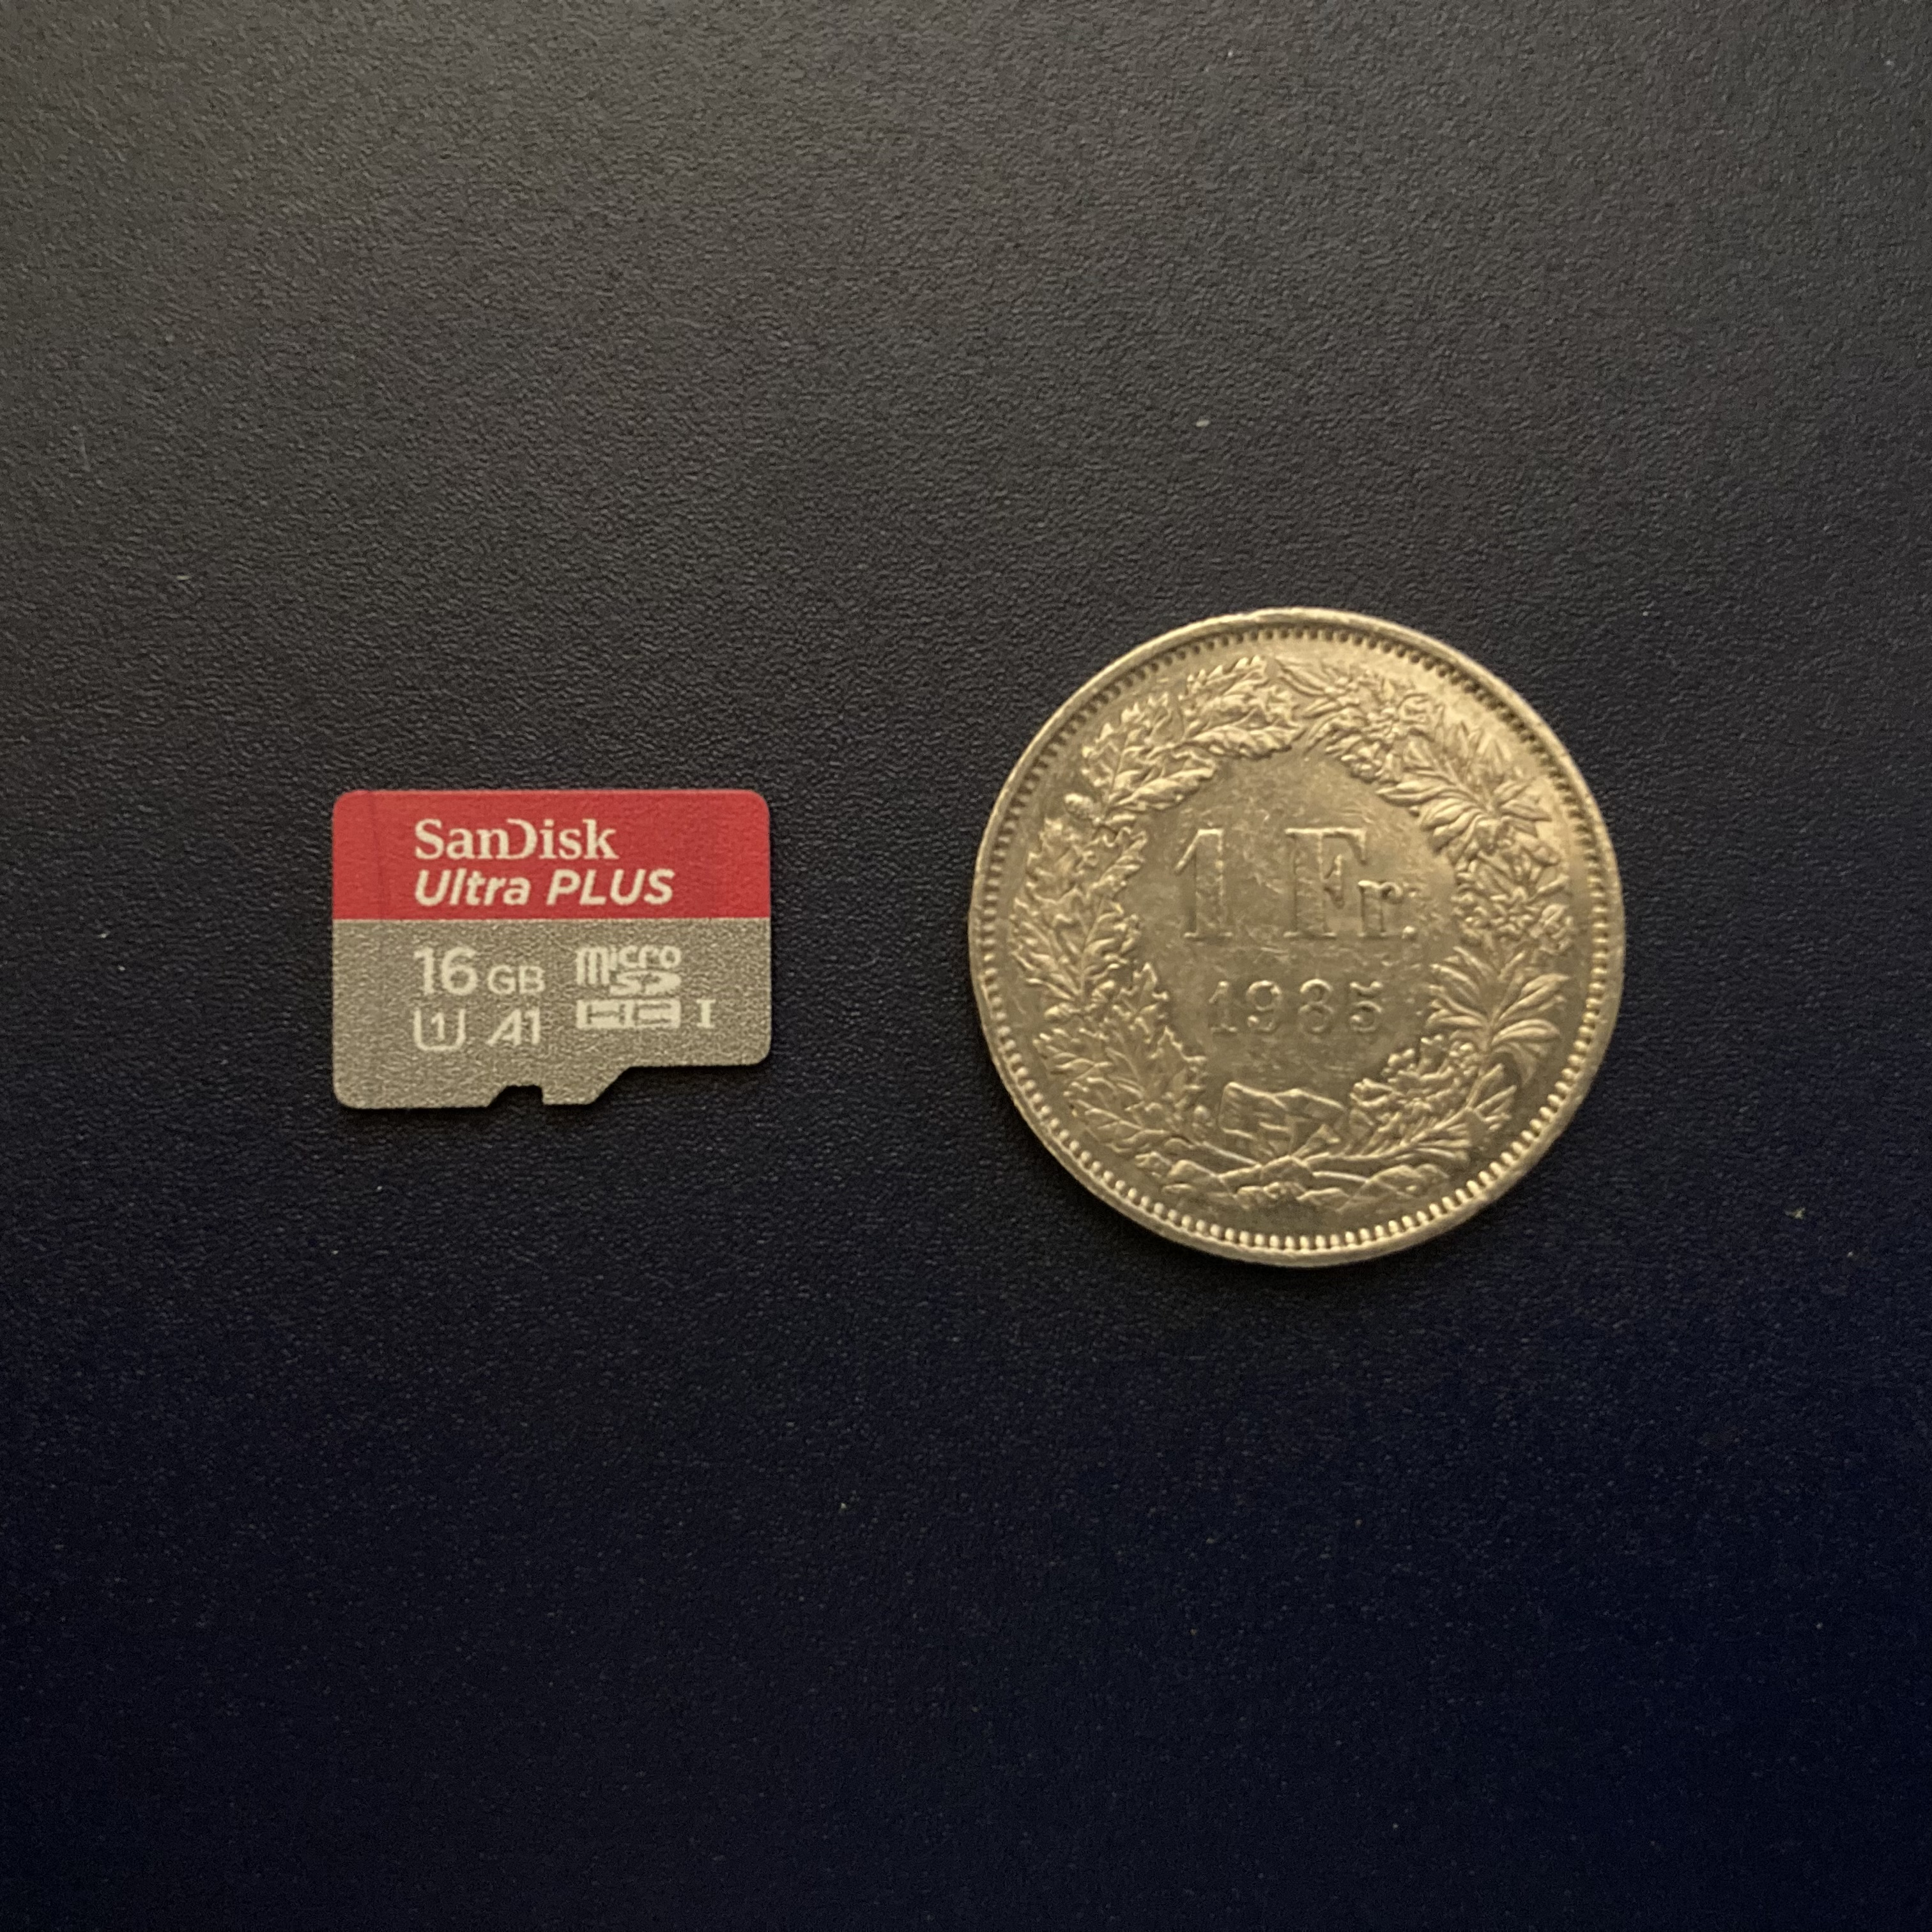
\includegraphics[width=0.25\textwidth]{images/hardware/microSD.jpeg}
    \caption{Carte micro SD à côté d'une pièce de 1 franc pour l'échelle}
    \label{fig:microsd}
\end{wrapfigure}
Il a fallu ensuite installer un système d'exploitation sur la carte SD. Nous avons donc suivi les instructions de la documentation officielle\footnote{\url{https://www.raspberrypi.com/documentation/computers/getting-started.html\#installing-the-operating-system}}, et avons installé \textit{Raspberry Pi Imager} sur l'ordinateur de Daniel. Puis, nous avons sélectionné le système d'exploitation \textit{Raspberry Pi OS Lite (32-bit)}, car notre modèle à une architecture en \textit{arm32} \cite{arm32} et que nous n'avions pas besoin d'un environnement de bureau \cite{desktopenv}. Ensuite, nous avons installé et paramétré le programme \mintinline{text}{ssh} \cite{ssh}, afin de pouvoir accéder à la carte à distance. Finalement, l'avons configurée pour qu'elle puisse émettre son propre réseau Wifi, en suivant à nouveau les instructions officielles\footnote{\url{https://www.raspberrypi.com/documentation/computers/configuration.html\#setting-up-a-routed-wireless-access-point}}. Par ailleurs, Daniel avait constaté une faute de frappe sur la documentation. Mais comme le site était Open Source \cite{opensource}, il a simplement fait une pull request, qui a été acceptée quelques jours après.\footnote{\url{https://github.com/raspberrypi/documentation/commit/e7e2d7ffcba31cf6ad233fc4a70dbfe623a820f4}} \\
Pour finir, la carte créait un réseau Wifi. Il ne restait plus "que" à faire le jeu. 

\subsection{Tutoriel de Tom Weiland}
Nous avions tous les deux déjà programmé des jeux, mais nous n'avions aucune expérience des jeux en ligne. Nous avons donc étudié les différentes façons d'en créer un avec Unity, le moteur de jeu que nous souhaitions utiliser. Il existait de nombreuses solutions offertes directement par la plateforme, mais la plupart ne semblaient pas assez complexes pour nos besoins et leurs critiques étaient plutôt négatives. De plus, la plupart utilisaient \textit{Unity Server,} mais ce programme ne pouvait pas se compiler pour l'architecture de la Raspberry (arm32 \cite{arm32}). Il était aussi très lourd et ne nous paraissait pas nécessaire pour notre utilisation.\\
C'est ainsi que nous avons découvert le youtubeur Tom Weiland et son fabuleux tutoriel \cite{tomweiland} sur le Networking en C\#. Son projet était basé sur \textit{.NET} \cite{dotnet}, qui utilise le même langage que Unity.  \\
Cependant, nous avons quand même dû l'adapter à nos besoins. En effet, son client était en 3D, tandis que nous voulions faire un jeu en 2D. De plus, il a fallu changer l'interface utilisateur, les graphismes, ainsi que, le fonctionnement du jeu lui-même. La figure \ref{fig:tutorial} montre ce tutoriel.
\begin{figure}
	\centering
    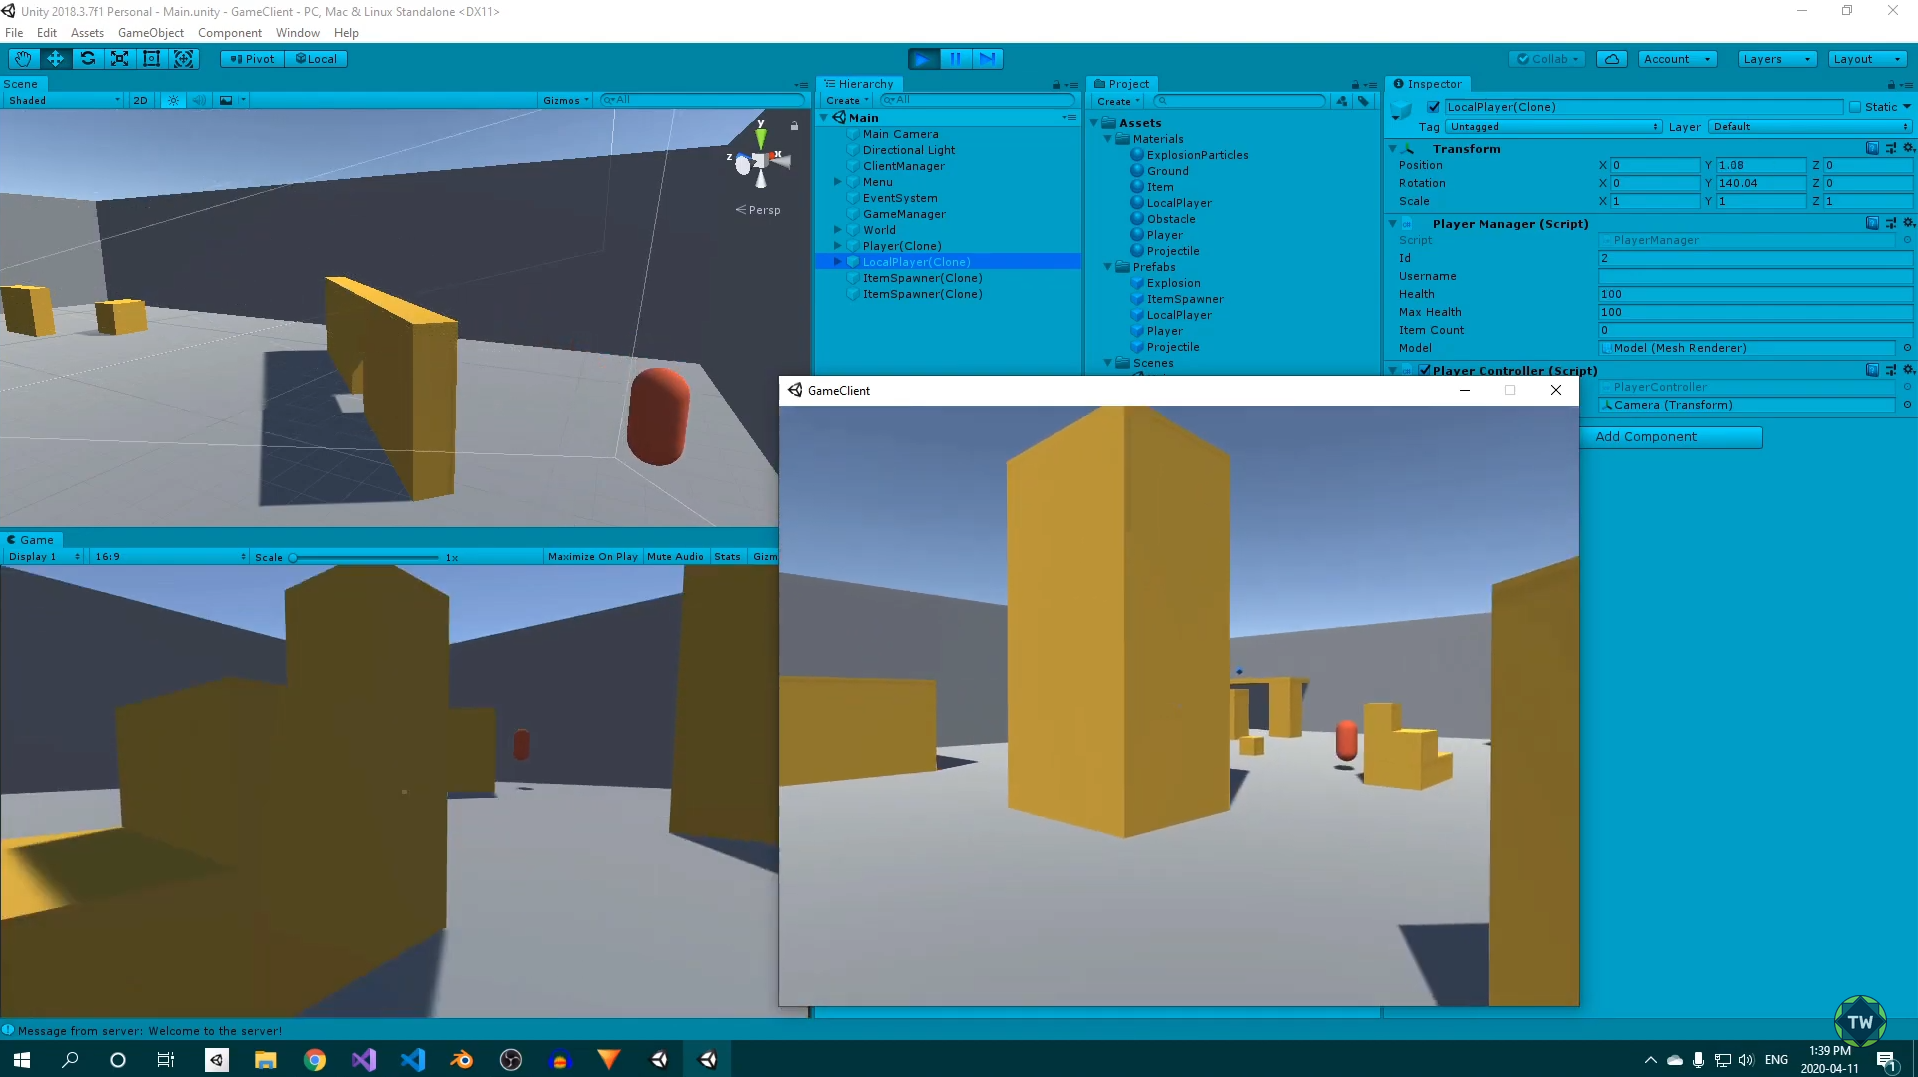
\includegraphics[width=0.9\textwidth]{images/tutorial.png}
    \caption{Jeu de Tom Weiland.}
    \label{fig:tutorial}
\end{figure}

\subsection{Chronologie}
\subsubsection{9 Mars 2022}
Comme dit précédemment, c'est à cette date que nous avons reçu la Raspberry Pi

\subsubsection{17 Mars 2022}
C'est à ce moment-là que nous avons réorganisé le projet, qui était originalement consacré à la création du Wifi, pour qu'il corresponde à la structure du tutoriel. 

\subsubsection{18 Mars 2022}
Création de notre \textit{Trello} \cite{trello}. La figure \ref{fig:trello} montre une capture d'écran de son état à la fin du projet.
\begin{figure}[h]
    \centering
    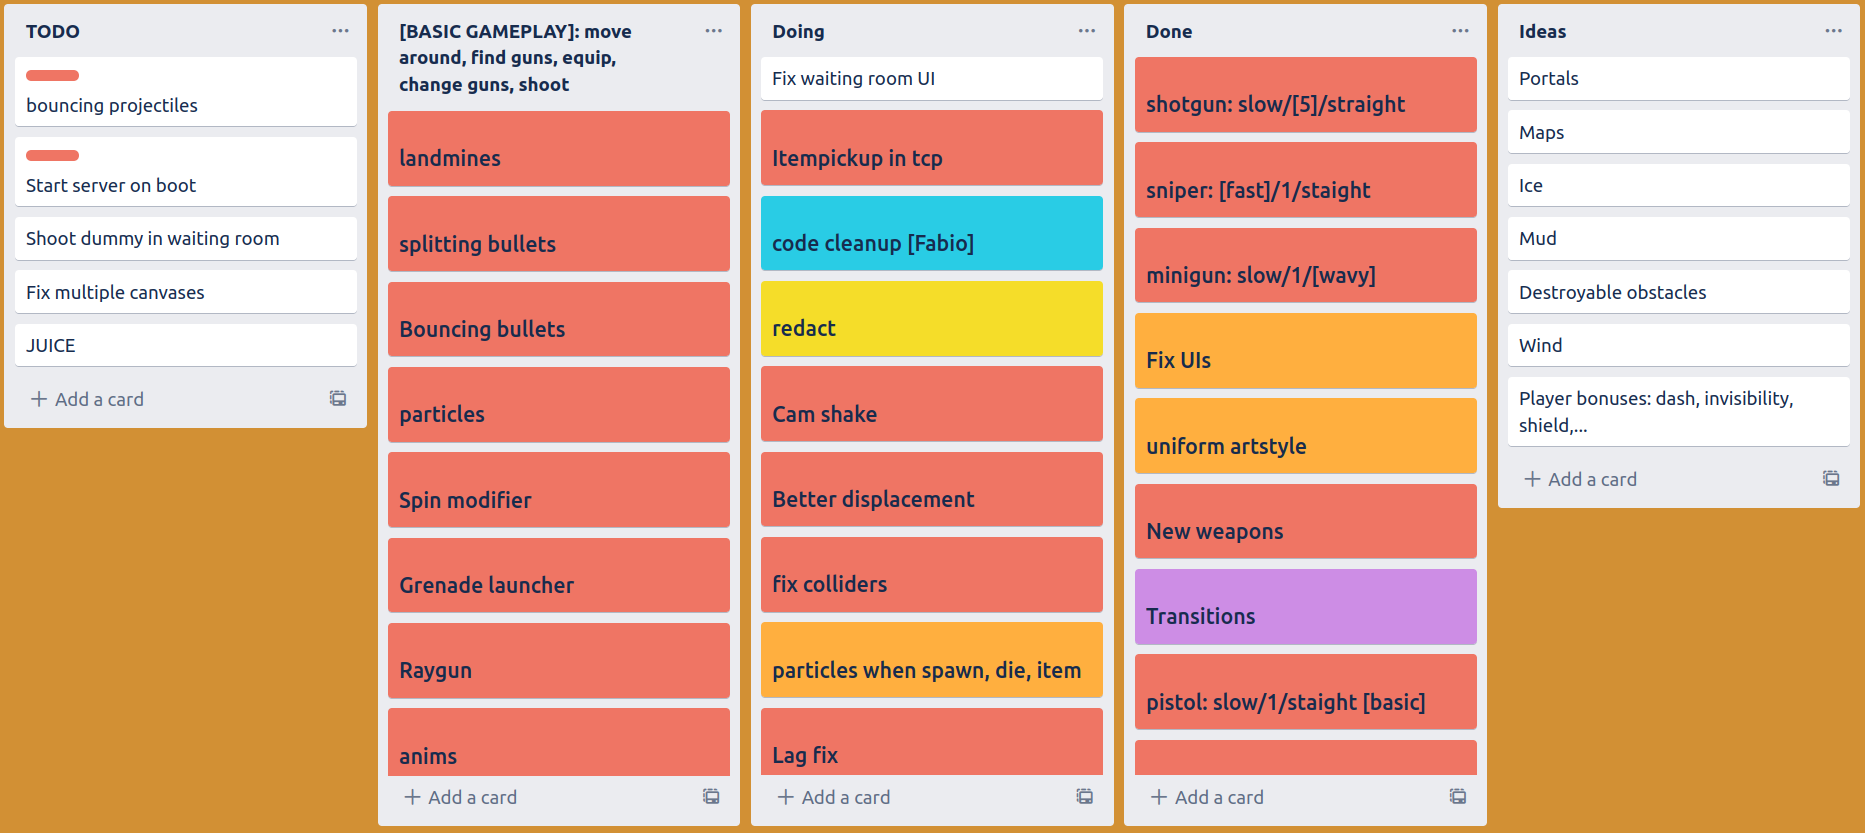
\includegraphics[width=\textwidth]{images/trello.png}
    \caption{Capture d'écran de notre \textit{Trello} à la fin du projet.}
    \label{fig:trello}
\end{figure}

\subsubsection{22 Mars 2022}
À cette date, Fabio a pu rejoindre le projet, car en raison d'un manque de temps et de divers problèmes techniques, il n'a pas pu le faire avant. Il ajouta donc les personnages qu'il avait dessinés, visibles à la figure \ref{fig:players},  avec le \textit{commit} "[Fabio] joined the game"\footnote{\url{https://github.com/DanielRoulin/Waypoint/commit/1bb1d6869941d451d384b7a802145543b2b81c72}}. (Les personnages n'ont pas été intégrés dans la version finale, voir la section \ref{artstyle} pour plus d'informations). Nous avons aussi expérimenté notre premier \textit{merge conflict}, car nous utilisions différentes versions d'Unity. C'est aussi à ce moment-là que nous avons fini de suivre le tutoriel et que nous avons commencé à travailler sur notre jeu, notamment en créant un script pour importer les scènes Unity sur notre serveur.

\begin{figure}
	\centering
    
\includegraphics[width=0.25\textwidth]{images/players/back.png}
    
\includegraphics[width=0.25\textwidth]{images/players/side.png}
    
\includegraphics[width=0.25\textwidth]{images/players/forward.png}
    \caption{Dessins de joueurs par Fabio}
    \label{fig:players}
\end{figure}

\subsubsection{22 au 28 Mars 2022}
Entre ces deux dates, nous avons ajouté les animations des joueurs et les objets qui deviendront plus tard les armes. Fabio a commencé à travailler sur les trajectoires des projectiles. De plus, Daniel a ajouté le \textit{parsing} des scènes sur le serveur.

\subsubsection{28 Mars au 1 Mai 2022}
Durant cette période, nous avons principalement travaillé sur les mécaniques de base, telles que la réapparition des joueurs, la salle d'attente et les conditions de début et de fin d'une partie. Nous avons aussi commencé à améliorer l'interface utilisateur.

\subsubsection{1 au 14 Mai 2022}
Durant cette période, nous avons ajouté les collisions au serveur, créé toutes les \textit{maps} actuelles, visibles sur la figure \ref{fig:maps}, avec le \textit{tileset} \cite{tileset} de Fabio. Nous avons continué à travailler sur l'interface du client et essayé d'automatiser la compilation du client et du serveur avec \textit{Github Action}\footnote{Github Action est un service proposé par Github permettant d'exécuter du code sur leur serveur à chaque \textit{commits}.},  ce qui n'a malheureusement pas abouti, car ce système était trop complexe et n'était pas adapté à nos besoins. Nous avons aussi corrigé des bugs mineurs que nous avions trouvés.

\begin{figure}
	\centering
    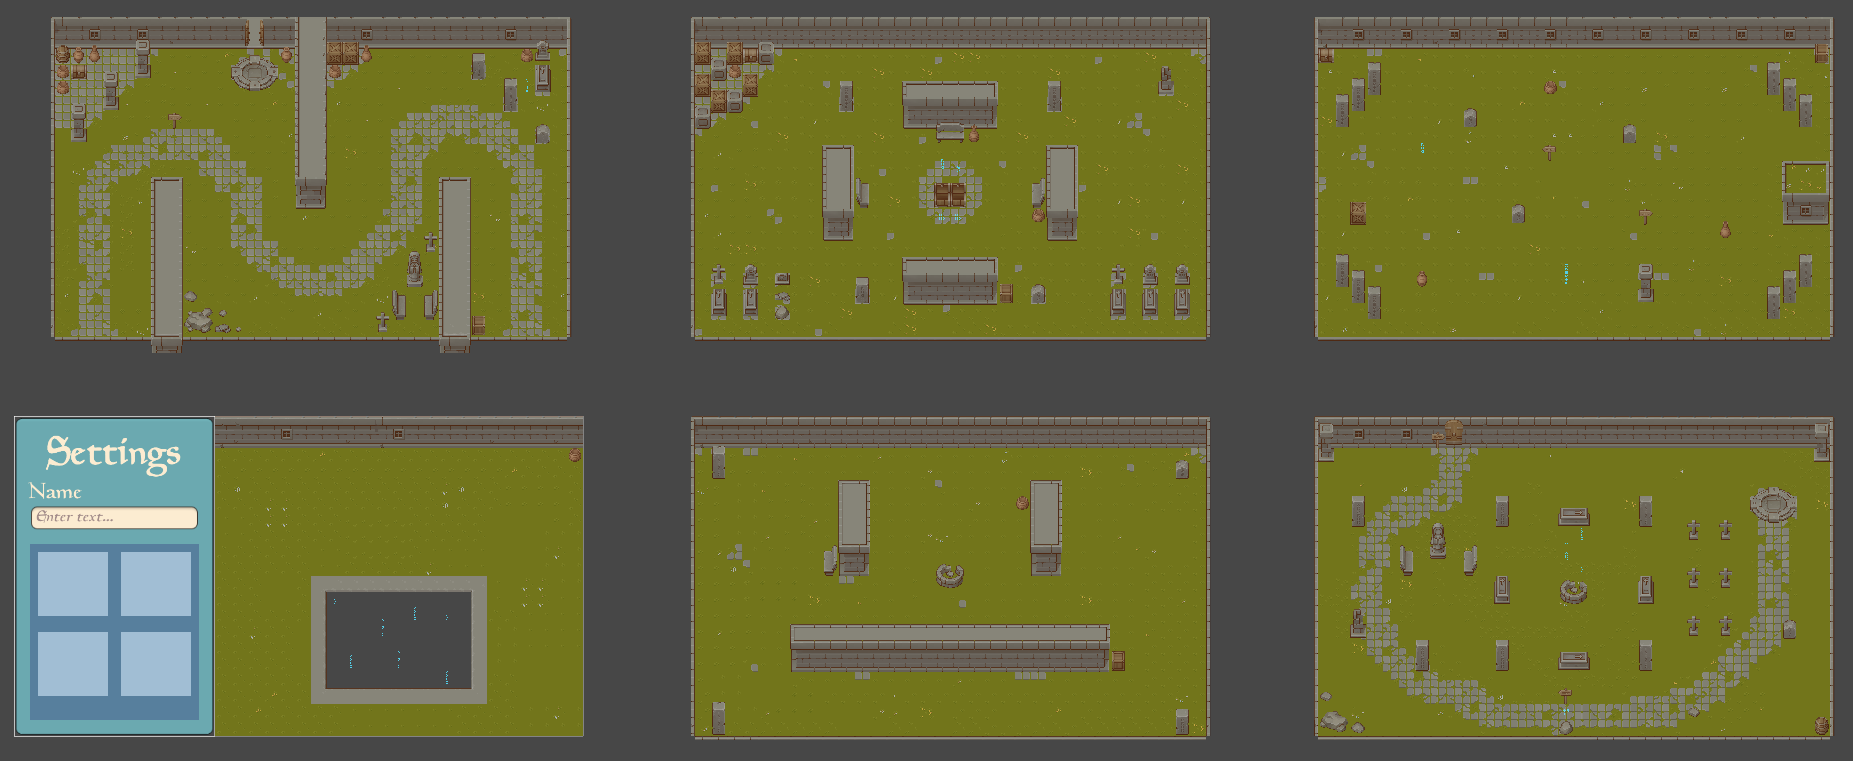
\includegraphics[width=0.9\textwidth]{images/game/maps.png}
    \caption{Différentes cartes de jeux}
    \label{fig:maps}
\end{figure}


\subsubsection{11 au 29 Août 2022}
Après deux mois de pause pendant les vacances d'été, nous avons continué à travailler sur le projet. Pour commencer, Fabio a ajouté beaucoup d'armes et d'objets et a créé un système modulaire permettant de créer des armes en fonction de différents paramètres. Puis, Daniel a séparé les différentes \textit{maps} dans leur propre scène (fichier). Cela a aussi nécessité de récrire le code du serveur, et a été la cause de notre plus gros \textit{merge conflict}, comme nous pouvons le voir à la Figure \ref{fig:conflict}.

\begin{figure}
	\centering
    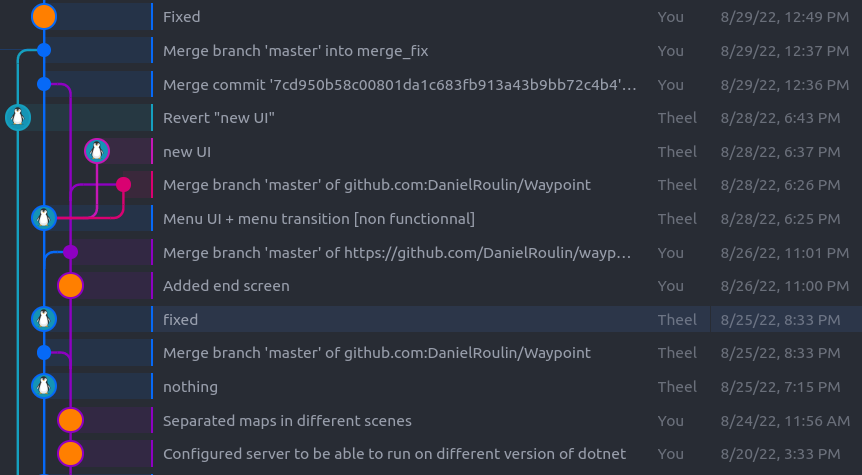
\includegraphics[width=0.9\textwidth]{images/conflict.png}
    \caption{Diagramme montrant les différentes branches du projet pendant le conflit}
    \label{fig:conflict}
\end{figure}
\subsubsection{30 Août au 19 Septembre}
Durant cette dernière période, nous n'avons pas ajouté de fonctionnalités majeures, mais nous nous sommes concentrés sur la correction de bugs, l'amélioration des menus, avec notamment l'ajout du menu \textit{option} et \textit{pause}, ainsi que des changements plutôt de l'ordre graphique. 

\subsubsection{19 Septembre à début Novembre}
En cette période, nous avons rédigé notre rapport, nettoyé le code et les fichiers du projet et nous avons fait les statistiques de la section \ref{section:chiffres}.

\newpage
\section{Problèmes rencontrés}
\subsection{FPS du serveur}
Le premier problème rencontré a été un problème d'optimisation. En effet, le serveur est un programme relativement simple qui peut être facilement exécuté par l'ordinateur. Mais cette facilité faisait que le programme était exécuté plusieurs centaines de fois par seconde, ce qui prenait trop de performances (mémoire, processeur, etc) et empêchait une bonne synchronisation entre le serveur et les clients. La solution était simple, il a suffi de limiter le nombre d'exécutions par seconde à un nombre raisonnable avec le code ci-dessous qui "mets en pause" l'exécution du programme pour qu'il n'y ait qu'une exécution par 30\textsuperscript{ème} de seconde:

\begin{listing}[!h]
\begin{minted}{csharp}
while (isRunning)
{
    while (_nextLoop < DateTime.Now)
    {
        GameLogic.Update();
        _nextLoop = _nextLoop.AddMilliseconds(Constants.MS_PER_TICK);
        if (_nextLoop > DateTime.Now)
        {
            Thread.Sleep(_nextLoop - DateTime.Now);
        }
    }
}
\end{minted}
\caption{Code pour la limitation du nombre d'exécutions par seconde}
\label{extrait:fps}
\end{listing}

\subsection{Scene parsing}
Quand nous avons commencé à créer des cartes pour les joueurs, nous nous sommes rapidement heurtés à un problème: comment synchroniser les terrains du serveur avec ceux du client ? En effet, il est nécessaire que les deux connaissent la position des obstacles, des points d'apparition et des déclencheurs d'événement, le premier afin d'appliquer la logique du jeu, le deuxième dans le but d'afficher correctement ces éléments. La meilleure solution que nous avons trouvée consiste à ajouter des informations destinées au serveur sur les scènes du client, puis de les copier sur le serveur pour qu'il puisse les interpréter. Cependant, il n'existait pas de \textit{parser} \cite{parser} pour le format des scènes utilisé par Unity (UnityYaml \cite{unityyaml}). En revanche, comme son nom l'indique, le format est basé sur le YAML \cite{yaml}, pour lequel des libraires existent en C\#. Nous avons donc décidé de créer notre propre \textit{parser} par-dessus, que l'on peut trouver dans le fichier \emph{Scene.cs}.

\subsubsection{Format}
\begin{listing}[!h]
\begin{minted}{yaml}
%YAML 1.1
%TAG !u! tag:unity3d.com,2011:
--- !u!1 &835401395
GameObject:
  m_ObjectHideFlags: 0
  m_Component:
  - component: {fileID: 835401396}
  m_Name: Square (2)
  m_TagString: ServerCollideable
  m_IsActive: 1
--- !u!4 &835401396
Transform:
  m_ObjectHideFlags: 0
  m_GameObject: {fileID: 835401395}
  m_LocalRotation: {x: -0, y: -0, z: -0, w: 1}
  m_LocalPosition: {x: 0, y: 7.5, z: 0}
  m_LocalScale: {x: 30, y: 1, z: 1}
  m_Children: []
  m_Father: {fileID: 1928389500}
  m_RootOrder: 1
  m_LocalEulerAnglesHint: {x: 0, y: 0, z: 0}
\end{minted}
\caption{Example d'un fichier UnityYaml avec un seul GameObject.}
\label{extrait:scene}
\end{listing}
\noindent Comme on le voit dans l'extrait \ref{extrait:scene}, un fichier \textit{.unity} comporte d'abord un en-tête. De plus, ce fichier est composé d'une liste de fichiers \textit{Yaml} valides, séparés par un une courte chaîne de caractères contenant leur type et leur id. Chaque fichier \textit{Yaml} représente un composant de la scène. Chacun de ces composants sont liés entre eux par leur id pour former une hiérarchie cohérente. 

\subsubsection{Parsing}
Pour commencer, nous découpons le fichier par l'en-tête de chaque sous-fichiers, qui commence toujours par "\mintinline{text}{---}". Puis, nous parsons chaque fichier en utilisant la librairie YamlDotNet \cite{yamldotnet}. Ensuite, nous ajoutons le résultat à un dictionnaire, avec pour index son \mintinline{text}{object_id}. C'est la fonction \mintinline{csharp}{ParseObjects}, visible dans l'extrait \ref{extrait:parseobjects}. 
\begin{listing}[!ht]
\begin{minted}{csharp}
private void ParseObjects()
{
    string file = File.ReadAllText(path);
    string[] files_array = file.Split("--- ");
    List<string> files = files_array.ToList<string>();
    files.RemoveAt(0);

    objects = new Dictionary<string, dynamic>();
    foreach (var f in files)
    {
        string[] splits = f.Split("\n", 2);
        string header = splits[0];
        string document = splits[1];
        string object_id = header.Split("&")[1];

        objects[object_id] = ParseYaml(document);
    }
}
\end{minted}
\caption{Fonction \mintinline{csharp}{ParseObjects}.}
\label{extrait:parseobjects}
\end{listing} \\
Ensuite, dans la fonction \mintinline{csharp}{ParseScene}, visible dans l'extrait \ref{extrait:parsescene}, nous étudions chaque objets parsés et vérifions le \textit{tag} de chaque \mintinline{csharp}{GameObject}:
\begin{itemize}
\item Si c'est un \textit{ServerCollideable}, nous le transformons en un \textit{collider} du serveur avec la fonction \mintinline{csharp}{ObjectToCollider} et l'ajoutons à la liste d'obstacles de cette scène.
\item Si c'est un \textit{ServerTrigger}, nous le transformons aussi en \textit{collider} et assignons la variable \mintinline{csharp}{trigger}. Il ne peut donc y avoir qu'un seul \textit{trigger} par scène, et seule la scène {WaitingRoom} possède un trigger.
\item Si c'est un \textit{ServerSpawn}, nous utilisons la fonction \mintinline{csharp}{ObjectToVector2} pour le transformer en vecteur et ajoutons ce vecteur à la liste de points d'apparitions du serveur. 
\end{itemize}
\begin{listing}[H]
\begin{minted}{csharp}
foreach (KeyValuePair<string, dynamic> element in objects)
{
    string type = ((IDictionary<String, Object>)element.Value).Keys.First();

    if (type == "GameObject")
    {
        dynamic gameObject = element.Value.GameObject;
        string tag = gameObject["m_TagString"];

        switch (tag)
        {
            case "ServerCollideable":
                obstacles.Add(ObjectToCollider(gameObject));
                break;
            case "ServerTrigger":
                trigger = ObjectToCollider(gameObject);
                break;
            case "ServerSpawn":
                Vector2 spawn_position = ObjectToVector2(gameObject);                            
                mapSpawns.Add(spawn_position);
                break;
        }

    }
}
if (!obstacles.Any())
{
    throw new Exception($"No obstacles found in scene {path}");
}
\end{minted}
\caption{Fonction \mintinline{csharp}{ParseScene}.}
\label{extrait:parsescene}
\end{listing}

\subsubsection{Fonctions ObjectToCollider et ObjectToVector2}
\begin{listing}[!h]
\begin{minted}{csharp}
private RectCollider ObjectToCollider(dynamic gameObject)
{
    foreach (var component in gameObject["m_Component"])
    {
        string fileID = component["component"]["fileID"];
        dynamic component_object = objects[fileID];
        string component_type = ((IDictionary<String, Object>)component_object).Keys.First();

        if (component_type == "Transform")
        {
            dynamic transform = component_object.Transform;
            if (float.Parse(transform["m_LocalRotation"]["x"]) != 0 ||
                float.Parse(transform["m_LocalRotation"]["y"]) != 0 ||
                float.Parse(transform["m_LocalRotation"]["z"]) != 0)
            {
                throw new Exception($"[Import Error]: GameObject {gameObject["m_Name"]} is rotated. This is not supported");
            }

            return new RectCollider(
                new Vector2(float.Parse(transform["m_LocalPosition"]["x"], CultureInfo.InvariantCulture), float.Parse(transform["m_LocalPosition"]["y"], CultureInfo.InvariantCulture)),
                new Vector2(float.Parse(transform["m_LocalScale"]["x"], CultureInfo.InvariantCulture), float.Parse(transform["m_LocalScale"]["y"], CultureInfo.InvariantCulture))
            );
        }
    }
    throw new Exception($"[Import Error]: GameObject {gameObject["m_Name"]} does not have a transform component");
}
\end{minted}
\caption{Fonction \mintinline{csharp}{ObjectToCollider}}
\label{extrait:objecttocollider}
\end{listing}
\noindent Dans cette fonction, qui apparaît dans l'extrait \ref{extrait:objecttocollider}, nous récupérons le composant \mintinline{csharp}{Transform} de l'objet reçu en entrée, qui contient des informations sur sa position, sa rotation et sa taille. Nous créons ensuite un \textit{collider} à partir de ces informations. Il est intéressant de noter l'utilisation du type \mintinline{csharp}{dynamic,} qui nous permet d'avoir des variables dont on ne connait pas le type, telle que le résultat du \textit{parsing}. De plus, les \textit{colliders} ne peuvent pas gérer les rotations, donc le programme rapporte une erreur si un objet en possède. Finalement, nous utilisons aussi l'option \mintinline{csharp}{CultureInfo.InvariantCulture} quand nous transformons la chaîne de caractères en nombre à virgule flottante. En effet, sans cette option, le programme fonctionnait sur l'ordinateur de Daniel, mais par sur celui de Fabio, car ce dernier était en français. La fonction \mintinline{csharp}{ObjectToCollider} est similaire à la précédente, sauf qu'elle renvoie un vecteur à deux dimensions plutôt qu'un \textit{collider}.

\subsubsection{Améliorations}
En rédigeant ce texte, nous avons réalisé qu'il était possible d'optimiser ce programme en n'utilisant le parser YAML que quand il est nécessaires. En effet, nous avons réalisé après coup que le type de composant est présent dans l'en-tête de chaque sous-fichier. Il serait donc possible de ne \textit{parser} que les fichiers de type \textit{GameObject} et \textit{Transform}.

\subsection{Tri du classement}
\begin{figure}[H]
	\centering
    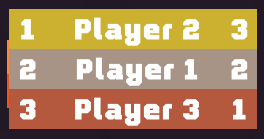
\includegraphics[width=0.4\textwidth]{images/game/leaderboard1.png}
    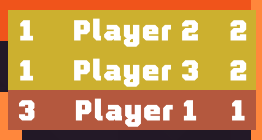
\includegraphics[width=0.4\textwidth]{images/game/leaderboard2.png}
    \caption{Images montrant le classement des joueurs, avec à droite une situation ou deux joueurs on le même score.}
    \label{fig:leaderboard}
\end{figure}

\newpage
\noindent Un problème que Daniel a rencontré en travaillant sur l'interface du client a été le suivant : comment trier et afficher le score des joueurs ? En effet, la solution naïve serait de simplement de trier les joueurs par ordre croissant et leur donner une position dans le classement correspondant à leur rang. Cependant, il se trouve que plusieurs joueurs peuvent avoir le même score, ce qui peut créer des erreurs ou afficher des entrées du classement par-dessus d'autre. De plus, le rang des joueurs peut ne pas être continu, comme on le voit à droite de la figure \ref{fig:leaderboard}. L'extrait \ref{extrait:leaderboard} montre la solution que nous avons trouvée. \\
\\
Pour commencer, nous utilisons les fonctions \mintinline{csharp}{GroupBy()} et \mintinline{csharp}{OrderByDescending()}, qui viennent du \textit{namespace} \cite{namespace} \mintinline{csharp}{System.Linq}. Ce \textit{namespace} permet  de facilement trier des listes et des dictionnaires. La première fonction permet de grouper les éléments d'une liste dans un dictionnaire, en fonction d'une condition. Ici, nous regroupons toutes les entrées avec le même score. La deuxième fonction nous permet de trier ces groupes par ordre décroissant de leurs scores.  \\
Durant la suite du programme, nous utilisons deux variables : \mintinline{csharp}{totalRank} et \mintinline{csharp}{rank}. \mintinline{csharp}{totalRank} est l'ordre apparent des entrées, tandis que \mintinline{csharp}{rank} correspond au rang affiché à droite des noms des joueurs (voir la figure \ref{fig:leaderboard}).  Ces deux valeurs sont initialisées à 1 au début du programme. Le reste du programme fonctionne de la façon suivante : \\
D'abord, on regarde chaque groupe trié. Puis, on donne à la variable \mintinline{csharp}{rank} la valeur de la variable \mintinline{csharp}{totalRank}. Cela permet d'avoir des rangs discontinus. Ensuite, pour chaque entrée du groupe, on met à jour son rang et sa couleur en fonction de la variable \mintinline{csharp}{rank} et de sa position en fonction de \mintinline{csharp}{totalRank}. Finalement, on ajoute 1 à la variable \mintinline{csharp}{totalRank}. \\
C'est donc en utilisant quelque fonction de triage et deux variables que nous arrivons à résoudre le problème apparemment simple du tri du classement.
\begin{listing}[H]
\begin{minted}{csharp}
public void SortLeaderboard()
{
    var grouped = entries.GroupBy(p => int.Parse(p.Value.kills.text));
    var ordered = grouped.OrderByDescending(g => g.Key);
    int totalRank = 1;
    foreach (var group in ordered)
    {
        var reorderedGroup = group.OrderBy(entry => entry.Value.username.text);
        int rank = totalRank;
        foreach (KeyValuePair<int, LeaderboardEntry> entry in reorderedGroup)
        {
            entry.Value.rank.text = rank.ToString();
            float y = entry.Value.rectTransform.rect.height/2 - totalRank*entry.Value.rectTransform.rect.height;
            entry.Value.targetPosition = new Vector2(0, y);
            totalRank++;
        }
    }
}
\end{minted}
\caption{Fonction \mintinline{csharp}{SortLeaderboard}, qui donne un rang et une position à chaque joueur en fonction de son score. Extrait tiré du fichier \mintinline{csharp}{Leaderboard.cs} du client.}
\label{extrait:leaderboard}
\end{listing}

\subsection{Sélection des points d'apparition}
\begin{listing}[H]
\begin{minted}{csharp}
public static Vector2 RandomFreeGoodPosition(float _radius)
{
    Vector2 bestPosition = Vector2.Zero;
    float bestDistance = 0f;
    for (int i = 0; i < 20; i++)
    {
        Vector2 _position = RandomFreeCirclePositionInMap(_radius);
        float smallestDistance = 10000f;
        foreach (Item item in Server.items.Values)
        {
            float distance = Vector2.Distance(item.position, _position);
            smallestDistance = MathF.Min(smallestDistance, distance);
        }
        foreach (Client client in Server.clients.Values)
        {
            if (client.player == null) continue;
            float distance = Vector2.Distance(client.player.position, _position);
            smallestDistance = MathF.Min(smallestDistance, distance);
        }
        if (bestDistance < smallestDistance)
        {
            bestDistance = smallestDistance;
            bestPosition = _position;
        }
    }
    return bestPosition;
}
\end{minted}
\caption{Fonction \mintinline{csharp}{RandomFreeGoodPosition}, qui permet de générer des bonnes positions pour l'apparition d'objets et de joueurs. Tiré du fichier  \mintinline{csharp}{Utilites.cs} du serveur.}
\label{extrait:position}
\end{listing}
\noindent
Au début de la création du jeu, nous faisions naïvement apparaître les joueurs et les objets en choisissant des coordonnées X et Y aléatoirement entre 0 et la largeur (ou la longueur) du terrain. Cependant, cette méthode comportait plusieurs problèmes. D'abord, il était possible que ces entités apparaissaient dans des obstacles, ce qui empêchait les joueurs de bouger et rendait les objets inaccessibles. Nous avions donc créé une fonction générant des positions aléatoires jusqu'à en trouver une qui n'intersectait aucun des obstacles de la scène. Cette solution permettait d'éviter le problème initial, mais en introduisait un autre : si un joueur est particulièrement malchanceux, il était possible qu'il apparaisse toujours désarmé en face d'un ennemi et que les armes se retrouvent toujours du côté de cet ennemi. Pour parer à cet inconvénient, nous avons rajouté une étape à la génération de positions, visible dans l'extrait \ref{extrait:position}. \\
Le fonctionnement de cette fonction est simple : on génère 20 positions grâce à la méthode précédemment expliquée, puis on choisit la position la plus loin de tout joueur et de toute arme. Pour ce faire, on commence par initialiser deux variables, \mintinline{csharp}{bestPosition} et \mintinline{csharp}{bestDistance}. Ces variables représentent la meilleure position et la plus grande distance trouvée à cet instant. Puis, pour chaque position, on regarde sa distance à l'objet ou le joueur le plus proche. Si cette distance est supérieure à \mintinline{csharp}{bestDistance}, alors \mintinline{csharp}{bestDistance} devient cette distance et \mintinline{csharp}{bestPosition} devient la position actuelle. \\
Cette méthode nous permet d'avoir une bonne distribution des entités sur le terrain. La qualité de cette distribution est en partie liée au nombre de positions testé. Dans notre cas, après quelques tests, 20 semblait être le meilleur compromis entre la qualité et la performance.

\subsection{Trajectoires des balles} 
Nous avons trouvé l'idée amusante que les joueurs puissent tirer des projectiles avec des trajectoires spéciales. La trajectoire la plus difficile à implémenter a été celle sinusoïdale, car nous ne comprenions pas comment implémenter cette fonctionnalité. Le problème a été résolu grâce au code ci-dessous qui, chaque 30\textsuperscript{ème} de seconde, modifie la trajectoire perpendiculaire à la direction de tir et lui donne la valeur du sinus de la distance entre la position de tir et la position de la balle. Le résultat est une balle qui avance et qui se balance de gauche à droite :


\begin{listing}[H]
\begin{minted}{csharp}
Vector2 dist = position - initialPos;
float totaldist = MathF.Abs(MathF.Sqrt(dist.X * dist.X + dist.Y * dist.Y));
Vector2 perp;
if (direction.Y == 0)
{
    perp = new Vector2(0, 1);
}
else
{
    perp = new Vector2(1, -direction.X / direction.Y);
}
float lenght = MathF.Sqrt(perp.X * perp.X + perp.Y * perp.Y);
perp = new Vector2(perp.X / lenght, perp.Y / lenght);
float crossZ = direction.X * perp.Y - perp.X * direction.Y;
if (crossZ < 0)
{
    perp = new Vector2(-perp.X, -perp.Y);
}
float mod = position.X / direction.X;
position += direction * speed * 2;
position += perp * speed * MathF.Cos(totaldist * frequency) * height;
\end{minted}
\caption{Code responsable de la trajectoire des balles sinusoïdale. Tiré du fichier  \mintinline{csharp}{Projectile.cs} du serveur.}
\label{extrait:projectile}
\end{listing}

\subsection{Style artistique}
\label{artstyle}
Bien que nous voulions à la base créer un jeu dans le style "pixel art", nous nous sommes plutôt dirigés vers un style "néon", plus simple, plus rapide à réaliser et mieux adapté à l'ambiance du jeu. Le style graphique a pu être renforcé grâce à du \textit{post-processing} (traitement d'image) qui donne au jeu un ton plutôt explosif et lumineux.

\begin{figure}[h]
    \begin{subfigure}{0.5\textwidth}
        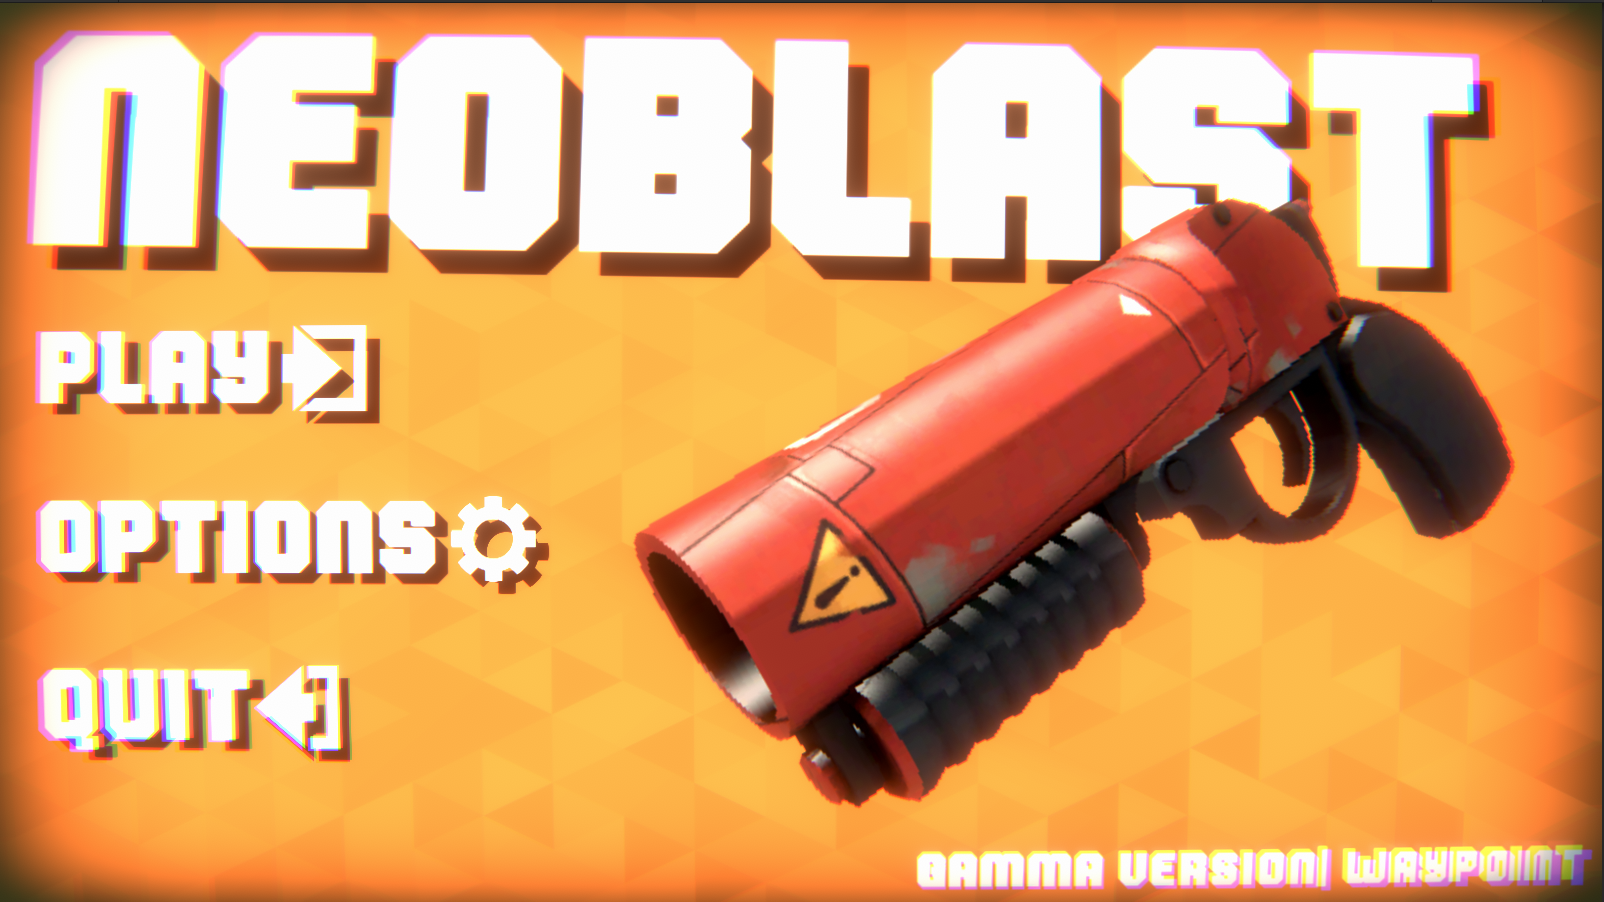
\includegraphics[width=0.9\textwidth]{images/game/start_menu.png}
        \caption{Jeu avec post-processing.}
        \label{fig:post_processing}
    \end{subfigure}
        \begin{subfigure}{0.5\textwidth}
        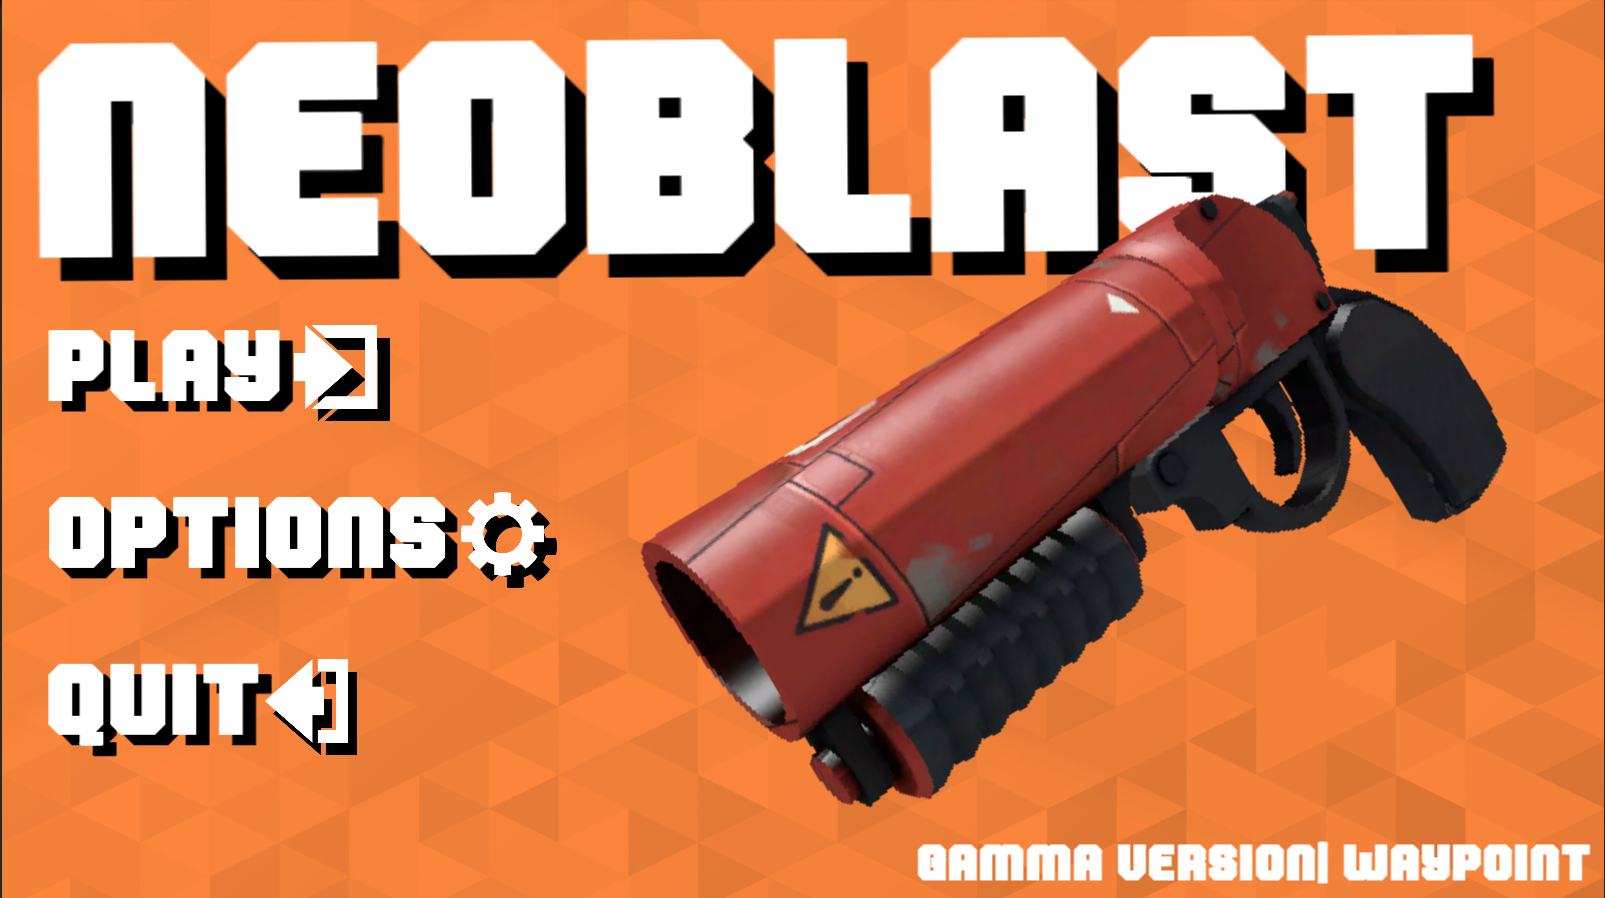
\includegraphics[width=0.9\textwidth]{images/game/no_postfx.png}
        \caption{Jeu sans post-processing.}
        \label{fig:no_post_processing}
    \end{subfigure}
\end{figure}

\section{Conclusion}
Ce projet nous a appris à utiliser de nouveaux outils, tel que le moteur de jeu Unity, qui était nouveau pour Daniel, le code en \textit{networking} et les systèmes de communication, ainsi que l'écriture en \LaTeX. En plus des connaissances techniques, ce projet nous a aussi appris à collaborer sur une longue période et à faire preuve de persévérance. \\
\\
Le projet a aussi un peu dévié par rapport à l'objectif initial.  L’idée originale prévoyait de faire un
jeu mobile, ce qui n’a pas été possible à cause de contraintes de temps. De plus, l'aspect de construction de sort a aussi été abandonnée et a été remplacé par le système d'arme.  La création d'un boîtier personnalisé a aussi dû être mise de côté, car la réalisation du jeu a pris plus de temps que prévu et Daniel a décidé de se concentrer sur ce dernier. Le style graphique du jeu a aussi été simplifié afin de dédier plus de temps aux fonctionnalités.\\
\\
En somme, nous sommes contents du résultat final; nous avons réussi à ouvrir une troisième voie dans le domaine du jeu multijoueur en créant un jeu local sur des appareils distincts. Nous sommes convaincus que cette idée à du potentiel pour de futurs projets, voire un avenir commercial.

\section{Remerciements}
Nous tenons à remercier toutes les personnes qui nous ont permis de venir à bout de ce projet: \\ 
M. Daniel Kessler, notre maître accompagnant, qui nous a conseillés, orientés et corrigés durant notre travail. \\
Nos parents, qui ont attentivement relu et corrigés ce document.  \\
Gérard Ineichen, qui nous a prêté du matériel indispensable. \\
Et bien sûr nos amis, qui ont participé au design et qui furent les premiers à essayer le jeu.









\newpage
\begin{thebibliography}{}
\bibitem{vps}
	Un VPS (Virtual Private Server) est un serveur dédié pouvant être loué au près d'hebergeurs web. Plus d'informations à cette addresse: \\
    \url{https://fr.wikipedia.org/wiki/Serveur_d\%C3\%A9di\%C3\%A9_virtuel}

\bibitem{dotnet}
	\textit{.NET} est une plateforme de développement dotée d'outils et de bibliothèques permettant de créer tout type d'application, notamment web, mobile, desktop, jeux, IoT, cloud et microservices. C'est la plateforme de notre serveur. Plus d'information à ces adresses: \\ 
    \url{https://dotnet.microsoft.com} \\
    \url{https://fr.wikipedia.org/wiki/.NET_Core}

\bibitem{tomweiland}
	Tom Weiland est un créateur de contenu et programmeur, connu notamment pour ses tutoriels sur Unity et surtout sur le networking en C\#, qui nous ont servis de base pour ce projet. Ci-joint l'adresse de son site web, son profil github et le tutoriel que nous avons suivi:
    \begin{itemize}
    	\item Site web: \url{https://tomweiland.net/}
        \item Github: \url{https://github.com/tom-weiland}
        \item Tutoriel: \url{https://youtube.com/playlist?list=PLXkn83W0QkfnqsK8I0RAz5AbUxfg3bOQ5}
    \end{itemize}

\bibitem{opensource}
	Du code est dit Open Source s'il est mis à disposition gratuitement pour d'éventuelles modifications et redistributions. Plus d'information à cette adresse: \\ 
    \url{https://en.wikipedia.org/wiki/Open_source}
    
\bibitem{build}
    En informatique, un build est la version compilé et exécutable d'un programme, contrairement au code source.

\bibitem{ssh}
	Le protocole Secure Shell (\mintinline{text}{ssh}) est un protocole de réseau cryptographique permettant d'exploiter des services réseau en toute sécurité sur un réseau non sécurisé. Ses applications les plus notables sont la connexion à distance et l'exécution de lignes de commande. Plus d'information à cette adresse: \\
    \url{https://fr.wikipedia.org/wiki/Secure_Shell}
    
\bibitem{raspberry}
	La Raspberry Pi est un nano-ordinateur monocarte à processeur ARM de la taille d'une carte de crédit conçu par des professeurs du 	  département informatique de l'université de Cambridge.
    Plus d'information à ces adresses: \\ 
    \url{https://fr.wikipedia.org/wiki/Raspberry_Pi}, \\
    \url{https://www.raspberrypi.org/help/what-\%20is-a-raspberry-pi/}
    
\bibitem{arm32}
      Les architectures ARM sont des architectures de type RISC 32 bits. Dotés d'une architecture relativement plus simple que d'autres familles de processeurs et faibles consommateurs d'électricité, les processeurs ARM sont aujourd'hui dominants dans le domaine de l'informatique embarquée. C'est l'architecture des Raspberry Pi.
      Plus d'information à cette adresse:\\
      \url{https://fr.wikipedia.org/wiki/Architecture_ARM}
      
 \bibitem{desktopenv}
 	En informatique, un environnement de bureau (de l'anglais \textit{desktop environment}) est l' interface utilisateur graphique qui ressemble à un bureau. 
    Plus d'information à cette adresse: \\
    \url{https://fr.wikipedia.org/wiki/Environnement_de_bureau}

\bibitem{git}
    Git permet de gérer les versions et de collaborer sur un projet. Plus d'information à cette adresse: \\
    \url{https://git-scm.com/}

\bibitem{unityyaml}
    UnityYAML est un format de fichier optimisé par Unity pour stocker des scènes, basé sur le format YAML (\url{https://yaml.org/}) mais ne supportant qu'un sous-ensemble des spécifications. Plus d'informations à cette adresse: \\
    \url{https://docs.unity3d.com/Manual/UnityYAML.html}
    
\bibitem{yamldotnet}
    YamlDotNet est une librairie pour la plateforme \textit{.NET} qui permet de parser du YAML. Nous l'utilisons pour l'interprétation des scènes sur le serveur. Plus d'informations à cette adresse: \\
    \url{https://github.com/aaubry/YamlDotNet}
    
\bibitem{parser}
	En informatique, un parser est programme qui prend des données d'entrée (souvent du texte) et les transforment en une représentation compréhensibles par l'ordinateur. Plus d'informations à cette adresse: \\
    \url{https://fr.wikipedia.org/wiki/Analyse_syntaxique}
    
\bibitem{yaml}
	YAML (YAML Ain't Markup Language) est un langage de sérialisation de données lisible par l'homme. Il est couramment utilisé pour les fichiers de configuration et dans les applications où les données sont stockées ou transmises. YAML ressemble dans son usage au JSON et XML. Il utilise l'indentation de style Python pour indiquer l'imbrication et est facilement extensible. Plus d'informations à cette adresse: \\
    \url{https://fr.wikipedia.org/wiki/YAML}
    
\bibitem{tcp}
    Le protocole TCP (Transmission Control Protocol) permet le transfert fiable de données entre ordinateurs sur le même réseau. Contrairement au protocole UDP, il est orienté sur des connections et garanti l'ordre des paquets. Documentation officielle accessible ici: \\
    \url{https://www.rfc-editor.org/rfc/rfc9293.html}
    
\bibitem{udp}
    Le protocole UDP (User Datagram Protocol) est un protocole permettant la transmission rapide de données entre ordinateurs sur le même réseau. UDP ne garantit ni l'ordre ni l'arrivée des paquets. Il est cependant bien plus rapide que le protocole TCP. Documentation officielle accessible ici: \\
    \url{https://www.rfc-editor.org/rfc/rfc768.html}
    
\bibitem{trello}
	Trello est un outil de gestion de projet en ligne. Il repose sur une organisation des projets en planches listant des cartes, chacune représentant des tâches. Les cartes sont assignables à des utilisateurs et sont mobiles d'une planche à l'autre, traduisant leur avancement. C'est l'outil que nous avons utilisé pour décider qui ferait quoi. Plus d'informations à ces adresses: \\
    \url{https://fr.wikipedia.org/wiki/Trello} \\
    \url{https://trello.com/fr}
    
\bibitem{tileset}
	Un tileset (ensemble de tuiles en français) est un ensemble d'images de même taille permettant de créer facilement des environnements.
    
\bibitem{namespace} 
  Les programmes C\# sont organisés à l’aide de \textit{namespace}. Ces derniers sont utilisés système d’organisation interne d'un programme et permettent de présenter les éléments de programme qui sont exposés à d’autres programmes. Plus d'informations à cette adresse: \\
  \url{https://learn.microsoft.com/fr-fr/dotnet/csharp/language-reference/language-specification/namespaces}

\end{thebibliography}






\newpage
\appendix
\section{Paquets}
\label{annexe:paquets}
\subsection{ServerPackets (envoyés du serveur au client)}
\paragraph{Welcome}
Premier message envoyé par le serveur, sert à donner un ID au client.
\begin{center}
\begin{tabular}{|p{1.5cm}|p{1.7cm}|p{1.9cm}|p{1.2cm}|p{6.7cm}|}
    \hline
    Packet Id & UDP/TCP & Nom & Type & Note \\
    \hline\hline
    \multirow{2}*{1} & \multirow{2}*{TCP} & message & string & Message de bienvenue, toujours défini comme "Welcome to the server!", utilisé uniquement pour débogage. \\
    \cline{3-5}
    & & clientId & int & Id du nouveau client \\
\hline
\end{tabular}
\end{center}

\paragraph{Spawn Player}
Envoyé par le serveur lorsqu' un nouveau  joueur rejoint la partie, aussi envoyé au joueur se connectant.
\begin{center}
\begin{tabular}{|p{1.5cm}|p{1.7cm}|p{1.9cm}|p{1.2cm}|p{6.7cm}|}
    \hline
    Packet Id & UDP/TCP & Nom & Type & Note \\
    \hline\hline
    \multirow{4}*{2} & \multirow{4}*{TCP} & client id & int & ID du joueur (identique à son ID client) \\
    \cline{3-5}
    & & username & string & Nom du joueur \\
    \cline{3-5}
    & & position & Vector2 & Position du joueur(0:0 représente le milieu de l’écran) \\
    \cline{3-5}
    & & rotation & float & Rotation de l’arme du joueur, en degré, sens trigonométrique, 0o est à l’horizontale à droite \\
    \hline
\end{tabular}
\end{center}

\paragraph{Disconnect Player}
Envoyé par le serveur aux joueurs restants lorsque un joueur averti le serveur qu’il se déconnecte.
\begin{center}
\begin{tabular}{|p{1.5cm}|p{1.7cm}|p{1.9cm}|p{1.2cm}|p{6.7cm}|}
    \hline
    Packet Id & UDP/TCP & Nom & Type & Note \\
    \hline\hline
    \multirow{1}*{3} & \multirow{1}*{TCP} & \multicolumn{3}{|l|}{(aucun)} \\
    \hline
\end{tabular}
\end{center}

\paragraph{Set Name}
Envoyé par le serveur à tous les joueurs lorsqu'un joueur change son nom.
\begin{center}
\begin{tabular}{|p{1.5cm}|p{1.7cm}|p{1.9cm}|p{1.2cm}|p{6.7cm}|}
    \hline
    Packet Id & UDP/TCP & Nom & Type & Note \\
    \hline\hline
    \multirow{2}*{4} & \multirow{2}*{TCP} & client id & int & ID du joueur \\
    \cline{3-5}
    & & username & string & Nom du joueur \\
    \hline
\end{tabular}
\end{center}

\paragraph{Start Game}
Envoyé par le serveur à tous les joueurs au début d’une partie
\begin{center}
\begin{tabular}{|p{1.5cm}|p{1.7cm}|p{1.9cm}|p{1.2cm}|p{6.7cm}|}
    \hline
    Packet Id & UDP/TCP & Nom & Type & Note \\
    \hline\hline
    \multirow{2}*{5} & \multirow{2}*{TCP} & duration & float & Durée de la partie, en secondes \\
    \cline{3-5}
    & & map id & int & ID de la map, >0 car 0 représente la salle d’attente. \\
    \hline
\end{tabular}
\end{center}

\paragraph{End Game}
Envoyé par le serveur à tous les joueurs à la fin d’une partie
\begin{center}
\begin{tabular}{|p{1.5cm}|p{1.7cm}|p{1.9cm}|p{1.2cm}|p{6.7cm}|}
    \hline
    Packet Id & UDP/TCP & Nom & Type & Note \\
    \hline\hline
    \multirow{1}*{6} & \multirow{1}*{TCP} & \multicolumn{3}{|l|}{(aucun)} \\
    \hline
\end{tabular}
\end{center}

\paragraph{Game Time}
Envoyé par le serveur à chaque tic pour les informer du temps restant.
\begin{center}
\begin{tabular}{|p{1.5cm}|p{1.7cm}|p{1.9cm}|p{1.2cm}|p{6.7cm}|}
    \hline
    Packet Id & UDP/TCP & Nom & Type & Note \\
    \hline\hline
    \multirow{1}*{7} & \multirow{1}*{UDP} & \multicolumn{3}{|l|}{(aucun)} \\
    \hline
\end{tabular}
\end{center}

\paragraph{Player Position}
Envoyé par le serveur à tous les joueurs lorsqu'un joueur bouge.
\begin{center}
\begin{tabular}{|p{1.5cm}|p{1.7cm}|p{1.9cm}|p{1.2cm}|p{6.7cm}|}
    \hline
    Packet Id & UDP/TCP & Nom & Type & Note \\
    \hline\hline
    \multirow{2}*{8} & \multirow{2}*{UDP} & client id & int & ID du joueur \\
    \cline{3-5}
    & & position & Vector2 & Position du joueur \\
    \hline
\end{tabular}
\end{center}

\paragraph{Player Rotation}
Envoyé par le serveur à tous les joueurs lorsqu'un joueur tourne.
\begin{center}
\begin{tabular}{|p{1.5cm}|p{1.7cm}|p{1.9cm}|p{1.2cm}|p{6.7cm}|}
    \hline
    Packet Id & UDP/TCP & Nom & Type & Note \\
    \hline\hline
    \multirow{2}*{9} & \multirow{2}*{UDP} & client id & int & ID du joueur \\
    \cline{3-5}
    & & rotation & float & Rotation du joueur \\
    \hline
\end{tabular}
\end{center}

\paragraph{Player Respawned}
Envoyé par le serveur à tous les joueurs lorsqu'un joueur réapparaît.
\begin{center}
\begin{tabular}{|p{1.5cm}|p{1.7cm}|p{1.9cm}|p{1.2cm}|p{6.7cm}|}
    \hline
    Packet Id & UDP/TCP & Nom & Type & Note \\
    \hline\hline
    \multirow{1}*{12} & \multirow{1}*{TCP} & \multicolumn{3}{|l|}{(aucun)} \\
    \hline
\end{tabular}
\end{center}

\paragraph{Player Hit}
Envoyé par le serveur à tous les joueurs lorsqu'un joueur est touché par un projectile.
\begin{center}
\begin{tabular}{|p{1.5cm}|p{1.7cm}|p{1.9cm}|p{1.2cm}|p{6.7cm}|}
    \hline
    Packet Id & UDP/TCP & Nom & Type & Note \\
    \hline\hline
    \multirow{2}*{10} & \multirow{2}*{TCP} & client id & int & ID du joueur touché \\
    \cline{3-5}
    & & by & int & ID du joueur ayant tiré le projectile \\
    \hline
\end{tabular}
\end{center}

\paragraph{Player Ammo}
Envoyé par le serveur au joueur lorsqu’il tire ou récupère une arme pour l’informer du nombre de balles qu’il possède.
\begin{center}
\begin{tabular}{|p{1.5cm}|p{1.7cm}|p{1.9cm}|p{1.2cm}|p{6.7cm}|}
    \hline
    Packet Id & UDP/TCP & Nom & Type & Note \\
    \hline\hline
    \multirow{1}*{11} & \multirow{1}*{TCP} & \multicolumn{3}{|l|}{(aucun)} \\
    \hline
\end{tabular}
\end{center}

\paragraph{Item Spawned}
Envoyé par le serveur à tous les joueurs lorsqu'un objet apparaît. 
\begin{center}
\begin{tabular}{|p{1.5cm}|p{1.7cm}|p{1.9cm}|p{1.2cm}|p{6.7cm}|}
    \hline
    Packet Id & UDP/TCP & Nom & Type & Note \\
    \hline\hline
    \multirow{3}*{13} & \multirow{3}*{TCP} & item id & int & ID de l’objet \\
    \cline{3-5}
    & & position & Vector2 & Position de l’objet \\
    \cline{3-5}
    & & type & int & Type de l’objet. (pistolet, fusil, mitraillette,...) \\
    \hline
\end{tabular}
\end{center}

\paragraph{Item Picked Up}
Envoyé par le serveur à tous les joueurs lorsqu'un objet est récupéré par un joueur. 
\begin{center}
\begin{tabular}{|p{1.5cm}|p{1.7cm}|p{1.9cm}|p{1.2cm}|p{6.7cm}|}
    \hline
    Packet Id & UDP/TCP & Nom & Type & Note \\
    \hline\hline
    \multirow{2}*{14} & \multirow{2}*{TCP} & item id & int & ID de l’objet \\
    \cline{3-5}
    & & client id & int & ID du joueur \\
    \hline
\end{tabular}
\end{center}

\paragraph{Projectile Spawned}
Envoyé par le serveur à tous les joueurs lorsqu'un projectile est tiré.
\begin{center}
\begin{tabular}{|p{1.5cm}|p{1.7cm}|p{1.9cm}|p{1.2cm}|p{6.7cm}|}
    \hline
    Packet Id & UDP/TCP & Nom & Type & Note \\
    \hline\hline
    \multirow{3}*{15} & \multirow{3}*{TCP} & projectile id & int & ID du projectile \\
    \cline{3-5}
    & & position & Vector2 & Position du projectile \\
    \cline{3-5}
    & & client id & int & ID du joueur qui a tiré le projectile \\
    \hline
\end{tabular}
\end{center}

\paragraph{Projectile Position}
Envoyé par le serveur à tous les joueurs lorsqu'un projectile bouge.
\begin{center}
\begin{tabular}{|p{1.5cm}|p{1.7cm}|p{1.9cm}|p{1.2cm}|p{6.7cm}|}
\hline
    Packet Id & UDP/TCP & Nom & Type & Note \\
    \hline\hline
    \multirow{2}*{16} & \multirow{2}*{UDP} & projectile id & int & ID du projectile \\
    \cline{3-5}
    & & position & Vector2 & Position du projectile \\
    \hline
\end{tabular}
\end{center}

\paragraph{Projectile Destroyed}
Envoyé par le serveur à tous les joueurs lorsqu'un projectile est détruit.
\begin{center}
\begin{tabular}{|p{1.5cm}|p{1.7cm}|p{1.9cm}|p{1.2cm}|p{6.7cm}|}
    \hline
    Packet Id & UDP/TCP & Nom & Type & Note \\
    \hline\hline
    \multirow{1}*{17} & \multirow{1}*{TCP} & \multicolumn{3}{|l|}{(aucun)} \\
    \hline
\end{tabular}
\end{center}

\subsection{Client Packets (envoyés du client au serveur)}
\paragraph{Welcome Received}
Premier message envoyé par le client, sert à confirmer l’ID du client.
\begin{center}
\begin{tabular}{|p{1.5cm}|p{1.7cm}|p{1.9cm}|p{1.2cm}|p{6.7cm}|}
    \hline
    Packet Id & UDP/TCP & Nom & Type & Note \\
    \hline\hline
    \multirow{1}*{1} & \multirow{1}*{TCP} & \multicolumn{3}{|c|}{(aucun)} \\
    \hline
\end{tabular}
\end{center}

\paragraph{Player Name}
Envoyé au serveur lorsque le joueur change son nom
\begin{center}
\begin{tabular}{|p{1.5cm}|p{1.7cm}|p{1.9cm}|p{1.2cm}|p{6.7cm}|}
    \hline
    Packet Id & UDP/TCP & Nom & Type & Note \\
    \hline\hline
    \multirow{1}*{2} & \multirow{1}*{TCP} & \multicolumn{3}{|c|}{(aucun)} \\
    \hline
\end{tabular}
\end{center}

\paragraph{Player Movement}
Envoyé au serveur à chaque tic, contient les boutons que le joueur presse ainsi que sa rotation.
\begin{center}
\begin{tabular}{|p{1.5cm}|p{1.7cm}|p{1.9cm}|p{1.2cm}|p{6.7cm}|}
    \hline
    Packet Id & UDP/TCP & Nom & Type & Note \\
    \hline\hline
    \multirow{3}*{3} & \multirow{3}*{UDP} & inputs length & int & Taille de la liste de boutons \\
    \cline{3-5}
    & & inputs & list [bool] & État des boutons: false = normal, true = pressé \\
    \cline{3-5}
    & & rotation & float & Rotation du joueur (angle entre l’horizon, le joueur et la souris) \\
    \hline
\end{tabular}
\end{center}

\paragraph{Player Shoot}
Envoyé au serveur quand le client clique.
\begin{center}
\begin{tabular}{|p{1.5cm}|p{1.7cm}|p{1.9cm}|p{1.2cm}|p{6.7cm}|}
    \hline
    Packet Id & UDP/TCP & Nom & Type & Note \\
    \hline\hline
    \multirow{1}*{4} & \multirow{1}*{TCP} & \multicolumn{3}{|c|}{(aucun)} \\
    \hline
\end{tabular}
\end{center}

\paragraph{Player End Game}
Envoyé au serveur quand le client appuie sur le bouton Continue quand la partie est finie. Signal au serveur que le joueur est prêt à jouer à nouveau.
\begin{center}
\begin{tabular}{|p{1.5cm}|p{1.7cm}|p{1.9cm}|p{1.2cm}|p{6.7cm}|}
    \hline
    Packet Id & UDP/TCP & Nom & Type & Note \\
    \hline\hline
    \multirow{1}*{5} & \multirow{1}*{TCP} & \multicolumn{3}{|c|}{(aucun)} \\
    \hline
\end{tabular}
\end{center}

\end{document}
